% =====================================================================
% Documento envoltorio para revisar y compilar los capitulos nuevos por
% separado, sin depender de la plantilla de la memoria.
%
% Compilar con:   latexmk -pdf memoria_capitulos_nuevos.tex
%
% Para integrarlos en la memoria definitiva basta con incluir
%   % =====================================================================
% CAPITULO 5 - RESULTADOS
% Sustituye al capitulo 5 de la version anterior de la memoria.
% Las tablas se generan con agentes/generar_tablas_latex.py y las figuras
% con agentes/generar_figuras_auditoria.py, ambas a partir de los CSV de
% los pasos 14-18. Ningun valor esta escrito a mano en este fichero salvo
% los citados en el texto corrido.
% =====================================================================

\section{Resultados}
\label{cap:resultados}

Este capítulo se organiza en torno a una distinción que resultó determinante:
la diferencia entre \emph{lo que un modelo consigue} y \emph{lo que una métrica
parece indicar}. Los cinco análisis que se presentan fueron especificados con su
hipótesis y su umbral de decisión fijados antes de ejecutarse. Dos de las cinco
hipótesis no se confirmaron, y se reportan como resultaron; mantener el criterio
original en esos dos casos es parte del resultado, no una concesión.

\subsection{Auditoría de integridad de las cohortes}
\label{sec:auditoria}

Antes de reevaluar cualquier modelo se auditó el estado real de los datos sobre
los que se construyeron los análisis. La tabla~\ref{tab:auditoria} resume las
once cohortes con datos procesados.

\begin{table}[htbp]
\centering
\caption[Auditoria de integridad de las cohortes]{Auditoria de integridad de
las once cohortes con datos procesados. La columna \emph{Desalin.} indica
muestras cuya etiqueta clinica corresponde a otro paciente por asignacion
posicional; \emph{Eval.} indica si la cohorte contiene ambas clases y por
tanto es evaluable como conjunto de test.}
\label{tab:auditoria}
\small
\begin{tabular}{llrrrrrcc}
\toprule
Cohorte & Plataforma & $n$ & Sanas & Enfermas & Sin clas. & Curacion & Desalin. & Eval. \\
\midrule
GSE118370 & GPL570 & 12 & 6 & 6 & 0 & 100,0\,\% & OK & si \\
GSE140797 & GPL13497 & 14 & 0 & 7 & 7 & 50,0\,\% & OK & \textbf{no} \\
GSE18842 & GPL570 & 91 & 45 & 46 & 0 & 100,0\,\% & OK & si \\
GSE19188 & GPL570 & 156 & 65 & 91 & 0 & 100,0\,\% & OK & si \\
GSE19804 & GPL570 & 120 & 60 & 60 & 0 & 100,0\,\% & OK & si \\
GSE23066 & GPL570 & 10 & 5 & 5 & 0 & 100,0\,\% & OK & si \\
GSE30219 & GPL570 & 307 & 0 & 307 & 0 & 100,0\,\% & \textbf{307/307} & \textbf{no} \\
GSE31210 & GPL570 & 246 & 20 & 226 & 0 & 100,0\,\% & OK & si \\
GSE40791 & GPL570 & 194 & 10 & 2 & 182 & 6,2\,\% & OK & si \\
GSE50081 & GPL570 & 181 & 0 & 181 & 0 & 100,0\,\% & OK & \textbf{no} \\
GSE7670 & GPL96 & 66 & 8 & 7 & 51 & 22,7\,\% & OK & si \\
\midrule
\textbf{Total} & & \textbf{1397} & 219 &
938 & \textbf{240} &
\textbf{82,8\,\%} & 307 & 8/11 \\
\bottomrule
\end{tabular}
\end{table}


La auditoría reveló cuatro problemas de naturaleza distinta.

\paragraph{Cobertura incompleta y silenciosa.} De las doce cohortes declaradas
en \texttt{datasets.txt}, tres nunca llegaron a procesarse: GSE40419, GSE81089 y
GSE140343, precisamente las tres basadas en RNA-seq. El fallo no generó ningún
error: el pipeline continuó y produjo resultados aparentemente completos. En
sentido inverso, dos cohortes presentes en los resultados (GSE118370 y
GSE140797) no figuran en el fichero de declaración. La cohorte efectivamente
analizada no coincide, por tanto, con la cohorte declarada.

\paragraph{Desalineamiento entre muestras y etiquetas clínicas.} En GSE30219,
las 307 columnas de la matriz de expresión están ordenadas de forma distinta a
las filas del fichero de metadatos, aunque ambos contengan el mismo conjunto de
muestras. Asignar las etiquetas por posición --- operación habitual cuando las
longitudes coinciden --- adjudica a cada muestra la información clínica de otro
paciente. El error afecta a la totalidad de la cohorte y no produce ninguna
señal de aviso.

Su efecto práctico se cuantificó de forma directa. Al entrenar el clasificador
de subtipo histológico (sección~\ref{sec:subtipo}) sobre los datos desalineados,
el AUC obtenido sobre esta cohorte fue de 0,56, indistinguible del azar. Con el
alineamiento corregido mediante identificador de muestra, el mismo modelo y los
mismos datos alcanzaron un AUC de 0,99. El desalineamiento no degrada el
resultado: lo destruye por completo, y lo hace de forma indistinguible de una
ausencia genuina de señal biológica.

\paragraph{Fallo parcial de la curación clínica automatizada.} La asignación de
etiquetas mediante modelo de lenguaje funcionó de forma completa en ocho de las
once cohortes, pero falló de manera severa en dos: en GSE40791 dejó sin
clasificar 182 de 194 muestras (93,8\,\%) y en GSE7670, 51 de 66 (77,3\,\%). En
conjunto, \sinclasificar{} de las \nmuestras{} muestras disponibles (\pctsinclasificar\,\%) quedaron fuera del
análisis por esta vía. La figura~\ref{fig:curacion} muestra la distribución por
cohorte. El patrón es relevante: el fallo no es gradual sino bimodal --- la
curación funciona casi perfectamente o se colapsa --- lo que sugiere
sensibilidad al formato concreto de los metadatos más que una limitación
uniforme de la capacidad del modelo.

\begin{figure}[htbp]
\centering
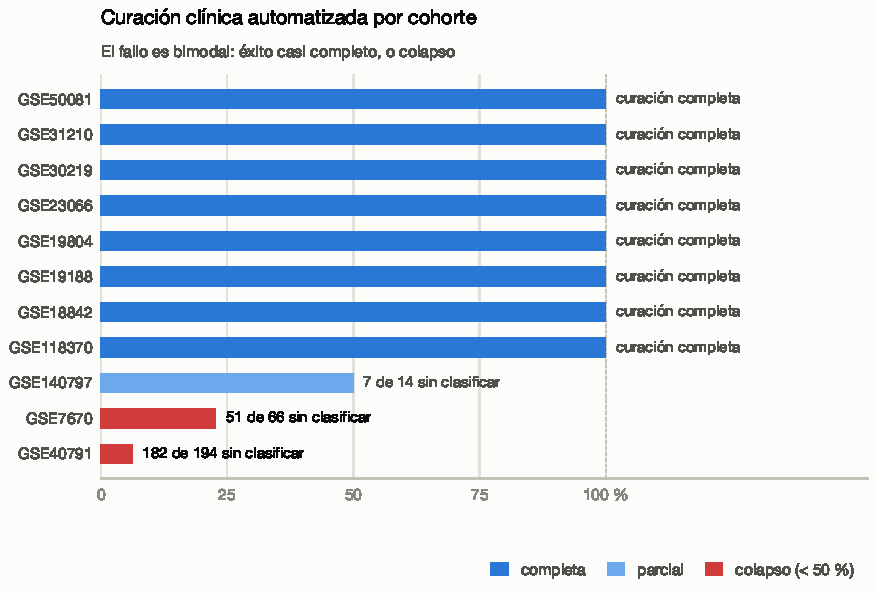
\includegraphics[width=0.95\textwidth]{figuras_auditoria/fig_curacion_llm.pdf}
\caption[Tasa de éxito de la curación automatizada]{Proporción de muestras a las
que la curación mediante modelo de lenguaje asignó una etiqueta utilizable. El
comportamiento es bimodal: éxito casi completo o colapso.}
\label{fig:curacion}
\end{figure}

\paragraph{Cohortes no evaluables empleadas como conjunto de test.} Tres
cohortes contienen únicamente muestras tumorales y ningún control: GSE30219
(307 muestras), GSE50081 (181) y GSE140797 (7). Una cohorte de una sola clase
puede formar parte legítimamente del conjunto de entrenamiento, pero no puede
funcionar como conjunto de test: en ella, la estrategia trivial de predecir
siempre la clase presente alcanza por definición una \emph{accuracy} de 1,000.
Cualquier valor elevado obtenido sobre estas cohortes es una consecuencia
aritmética de su composición, no una medida de capacidad predictiva.

\subsection{Reevaluación de la validación LODO}
\label{sec:lodo}

Se repitió la validación \emph{Leave-One-Dataset-Out} sobre la tarea tumor
frente a sano conservando deliberadamente el modelo original (regresión
logística con penalización $L_1$, $C=0{,}5$, sin ponderación de clases). Solo se
modificaron dos elementos: el alineamiento muestra--etiqueta y el conjunto de
métricas reportadas. Aislar así las variables permite atribuir cualquier
diferencia observada al modo de medir, y no a un cambio de método.

La hipótesis registrada fue que el rendimiento medio descendería respecto al
valor previamente reportado y que GSE31210 y GSE40791 quedarían por debajo de su
propio \emph{baseline}. La tabla~\ref{tab:lodo-honesto} recoge el resultado.

\begin{table}[htbp]
\centering
\caption[Validacion LODO con metricas completas]{Validacion LODO de la tarea
tumor frente a sano, con el mismo modelo del analisis original (LASSO, $C=0{,}5$)
y el alineamiento muestra--etiqueta corregido. Se anaden el \emph{baseline} de
clase mayoritaria y la \emph{balanced accuracy}; las tres cohortes con una sola
clase se marcan como no evaluables. En negrita, las cohortes que no superan su
propio \emph{baseline}.}
\label{tab:lodo-honesto}
\small
\begin{tabular}{lrcrrrrrr}
\toprule
Cohorte test & $n$ & Sano/Enf. & \emph{Baseline} & Acc. & Bal.\ acc. & AUC & Sens. & Espec. \\
\midrule
GSE118370 & 12 & 6/6 & 0,500 & 0,917 & 0,917 & 1,000 & 1,000 & 0,833 \\
GSE18842 & 91 & 45/46 & 0,505 & 0,890 & 0,889 & 1,000 & 1,000 & 0,778 \\
GSE19188 & 156 & 65/91 & 0,583 & 0,923 & 0,912 & 0,984 & 0,978 & 0,846 \\
GSE19804 & 120 & 60/60 & 0,500 & 0,775 & 0,775 & 0,984 & 1,000 & 0,550 \\
GSE7670 & 15 & 8/7 & 0,533 & 0,733 & 0,750 & 1,000 & 1,000 & 0,500 \\
GSE23066 & 10 & 5/5 & 0,500 & 0,500 & 0,500 & 0,440 & 1,000 & 0,000 \\
GSE31210 & 246 & 20/226 & 0,919 & 0,898 & 0,945 & 0,993 & 0,889 & 1,000 \\
GSE40791 & 12 & 10/2 & 0,833 & 0,167 & 0,500 & 1,000 & 1,000 & 0,000 \\
GSE50081 & 181 & 0/181 & 1,000 & 0,967 & \multicolumn{4}{c}{\emph{no evaluable: una sola clase}} \\
GSE30219 & 307 & 0/307 & 1,000 & 0,941 & \multicolumn{4}{c}{\emph{no evaluable: una sola clase}} \\
GSE140797 & 7 & 0/7 & 1,000 & 0,857 & \multicolumn{4}{c}{\emph{no evaluable: una sola clase}} \\
\midrule
\multicolumn{5}{l}{\emph{Media sobre las 8 cohortes evaluables}} &
\textbf{0,773} &
\textbf{0,925} &
0,983 & 0,563 \\
\multicolumn{5}{l}{\emph{Media de \emph{accuracy} sobre las 11 (como en el analisis original)}} &
\multicolumn{4}{c}{0,779} \\
\bottomrule
\end{tabular}
\end{table}


La hipótesis se confirmó. Sobre las ocho cohortes evaluables, la
\emph{balanced accuracy} media fue de \balacc{} y la ganancia media respecto al azar
informado, de $+$\gananciamedia{}. \nosuperan{} de las \nev{} cohortes evaluables no superan su
propio \emph{baseline}: GSE23066 lo iguala (\accaa{} frente a \baseaa{}), GSE31210
queda ligeramente por debajo (\accbb{} frente a \basebb{}) y GSE40791 lo hace de forma
drástica (\acccc{} frente a \basecc{}). La figura~\ref{fig:lodo} representa cada
cohorte frente a su umbral trivial.

\begin{figure}[htbp]
\centering
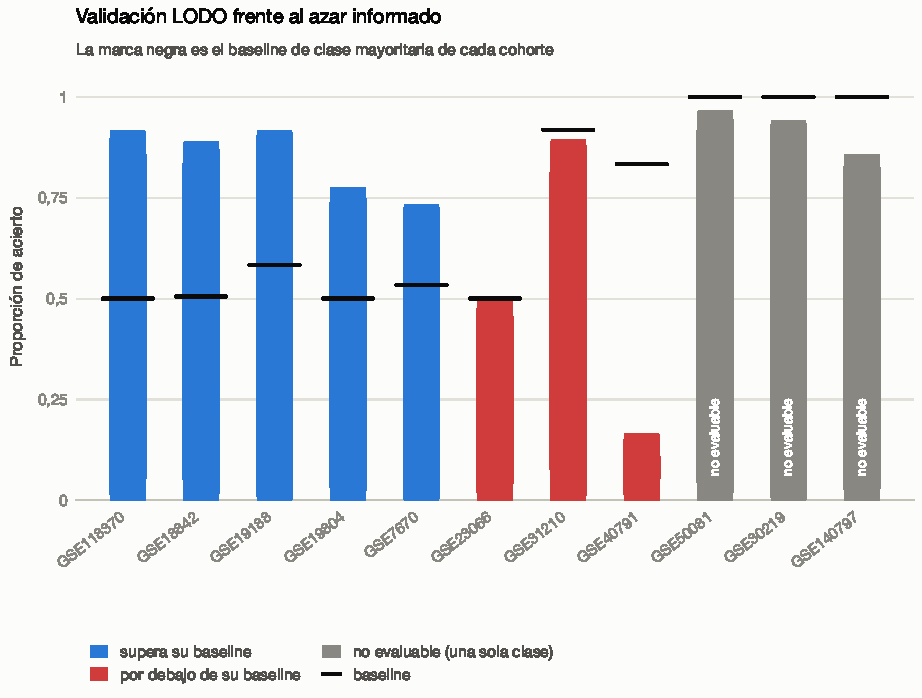
\includegraphics[width=\textwidth]{figuras_auditoria/fig_lodo_vs_baseline.pdf}
\caption[Validación LODO frente al azar informado]{\emph{Accuracy} obtenida en
cada cohorte externa (barras) frente al \emph{baseline} de clase mayoritaria
(marcas horizontales). En rojo, las cohortes evaluables que no superan su
umbral trivial; en gris, las tres cohortes de una sola clase, donde la métrica
carece de contenido.}
\label{fig:lodo}
\end{figure}

\subsubsection{Un hallazgo no previsto: discriminación sin decisión}
\label{sec:calibracion}

El análisis produjo un resultado que no formaba parte de la hipótesis registrada
y que resultó ser el más informativo del capítulo. Sobre las mismas ocho
cohortes evaluables, el AUC medio fue de \aucmedia{} mientras que la
\emph{balanced accuracy} media se quedó en \balacc{}. La divergencia entre ambas
métricas es sistemática, no anecdótica, y alcanza su expresión más extrema en
GSE40791: \emph{accuracy} de \acccc{} con un AUC de 1,000.

Un AUC de 1,000 indica que el modelo ordena perfectamente las muestras: existe
un umbral que las separa sin error. Una \emph{accuracy} de 0,167 indica que el
umbral empleado --- el valor por defecto de 0,5 --- no es ese. Las columnas de
sensibilidad y especificidad de la tabla~\ref{tab:lodo-honesto} identifican la
causa: la sensibilidad media es de \sensmedia{} y la especificidad media, de \especmedia{}. El
modelo clasifica como tumoral casi todo lo que recibe. Ese sesgo es coherente
con la composición del conjunto de entrenamiento, que reúne 938 muestras
tumorales frente a 219 controles.

La conclusión es que la firma transcriptómica sí transfiere entre cohortes
independientes en cuanto a su \emph{capacidad de ordenación}, pero el
\emph{punto de corte} no transfiere. La figura~\ref{fig:auc} representa ambas
dimensiones. Esta distinción tiene una consecuencia metodológica inmediata: los
valores de \emph{accuracy} próximos a 0,5 acompañados de un AUC próximo a 1,0
que aparecían en el análisis original no eran ruido ni indicios de dificultad
intrínseca del problema, sino la manifestación de un problema de calibración
enteramente corregible.

\begin{figure}[htbp]
\centering
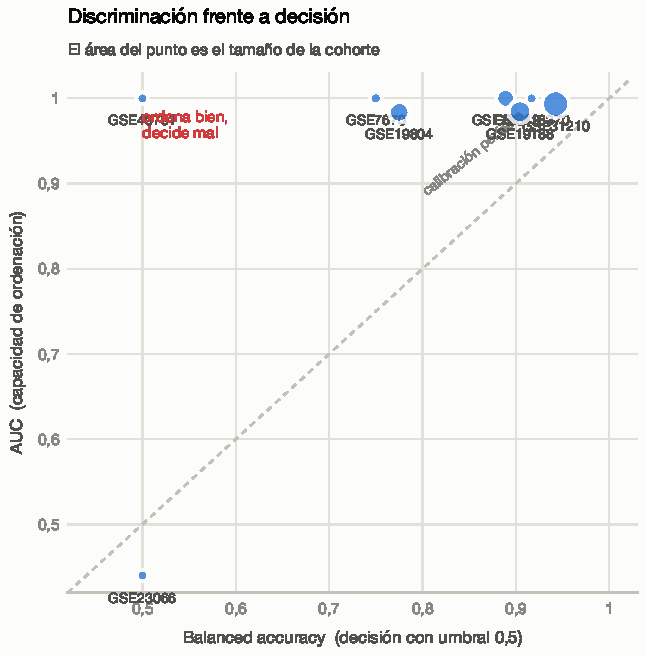
\includegraphics[width=0.62\textwidth]{figuras_auditoria/fig_auc_vs_balacc.pdf}
\caption[Discriminación frente a decisión]{Cada punto es una cohorte externa; el
tamaño es proporcional al número de muestras. La distancia a la diagonal mide
cuánto se pierde por un umbral de decisión mal calibrado. Las cohortes situadas
arriba a la izquierda ordenan bien y deciden mal.}
\label{fig:auc}
\end{figure}

\subsection{Naturaleza de la señal: composición tisular frente a biología tumoral}
\label{sec:composicion}

Los genes que encabezaban la firma de consenso previa sugerían una
interpretación alternativa a la de biomarcadores tumorales. Entre los cincuenta
primeros aparecen cinco marcadores canónicos de tejido pulmonar sano --- AGER y
CLDN18 (epitelio alveolar tipo~I), SFTPC (tipo~II), FABP4 y WIF1 --- todos con
un $\log$FC medio próximo a $-4$, junto con COL10A1, característico de estroma
desmoplásico, al alza. Ese perfil describe la sustitución de parénquima pulmonar
normal por tejido tumoral y estroma reactivo, es decir, una diferencia de
\emph{composición} de la muestra.

Para contrastarlo se construyó un \emph{score} de contenido de pulmón normal a
partir de un panel de 18 marcadores de compartimentos alveolar, endotelial y
estromal normal, y se correlacionó con el \emph{score} del clasificador. La
prueba decisiva se restringió a las muestras tumorales: sobre el conjunto
completo la correlación es alta por construcción, dado que los controles son
pulmón sano, y no distingue entre ambas hipótesis. El umbral fijado de antemano
fue $|\rho|>0{,}7$.

\begin{table}[htbp]
\centering
\caption[Composicion tisular frente a biologia tumoral]{Correlacion de Spearman
entre el \emph{score} del clasificador y el contenido de pulmon normal
(panel de 18 marcadores alveolares, endoteliales y de estroma normal). La
columna decisiva es la tercera: restringida a muestras tumorales, donde la
correlacion ya no puede explicarse por la presencia de controles sanos. Se
requieren al menos 8 tumores para calcularla.}
\label{tab:composicion}
\small
\begin{tabular}{lrrrrr}
\toprule
& & & \multicolumn{3}{c}{$\rho$ frente al \emph{score} del clasificador} \\
\cmidrule(l){4-6}
Cohorte & Tumores & Sanas & Todas (pulmon n.) & \textbf{Solo tumores} & Prolif. \\
\midrule
GSE31210 & 226 & 20 & $-$0,909 & $-$0,884 & 0,719 \\
GSE19188 & 91 & 65 & $-$0,826 & $-$0,347 & 0,416 \\
GSE19804 & 60 & 60 & $-$0,798 & $-$0,765 & 0,478 \\
GSE18842 & 46 & 45 & $-$0,874 & $-$0,550 & 0,267 \\
GSE7670 & 7 & 8 & $-$0,729 & \multicolumn{2}{c}{\emph{$n$ insuficiente}} \\
GSE118370 & 6 & 6 & $-$0,818 & \multicolumn{2}{c}{\emph{$n$ insuficiente}} \\
GSE23066 & 5 & 5 & $-$0,054 & \multicolumn{2}{c}{\emph{$n$ insuficiente}} \\
GSE40791 & 2 & 10 & $-$0,448 & \multicolumn{2}{c}{\emph{$n$ insuficiente}} \\
\midrule
\multicolumn{4}{l}{\emph{Media sobre las 4 cohortes evaluables}} &
\textbf{$-$0,637} &
0,470 \\
\bottomrule
\end{tabular}
\end{table}


\textbf{La hipótesis no se confirmó al umbral establecido.} La correlación media
entre muestras tumorales fue de $\rho=-\rhotumoresabs$, por debajo del criterio fijado,
y solo \nrhosupera{} de las \nrho{} cohortes con tumores suficientes lo superan
individualmente. El umbral no se ha modificado a posteriori.

La lectura que sostienen los datos es intermedia y más matizada que la
hipótesis de partida. La composición tisular explica una fracción sustancial de
la señal --- en GSE31210, la cohorte con más tumores evaluables ($n=226$), la
correlación alcanza $\rho=-0{,}870$ con $p=7\times10^{-71}$ --- pero no la
totalidad. Además, el análisis reveló un segundo eje no previsto: entre muestras
tumorales, el \emph{score} del clasificador correlaciona positivamente con un
panel de proliferación ($\rho$ entre $+\rhoprolifmin$ y $+\rhoprolifmax$). El clasificador
no lee un único fenómeno, sino al menos dos: cuánto parénquima normal conserva
la muestra y con qué intensidad proliferan sus células.

\begin{figure}[htbp]
\centering
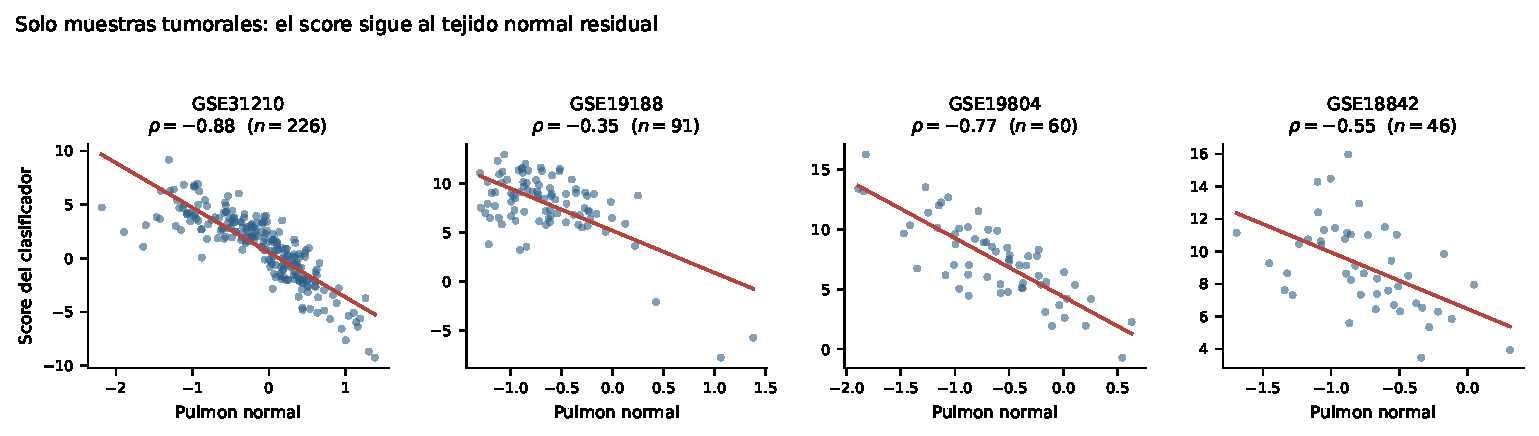
\includegraphics[width=\textwidth]{figuras_auditoria/fig_composicion_tumores.pdf}
\caption[Composición tisular dentro de los tumores]{Relación entre el
\emph{score} del clasificador y el contenido estimado de pulmón normal,
restringida a muestras tumorales. La pendiente negativa persiste al eliminar los
controles sanos, lo que indica que parte de la señal procede de tejido normal
residual y no de biología tumoral.}
\label{fig:composicion}
\end{figure}

\subsection{Validez de la consistencia de signo como medida de reproducibilidad}
\label{sec:falacia}

El análisis original cuantificaba la estabilidad de cada gen sumando el signo de
su coeficiente a lo largo de los \emph{folds} LODO, y presentaba valores como
$11/11$ como evidencia de robustez. Esta métrica presenta un problema
estructural: cada \emph{fold} entrena con todas las cohortes menos una, de modo
que dos \emph{folds} cualesquiera comparten la mayor parte de sus muestras de
entrenamiento. En la configuración analizada, la fracción compartida entre pares
de \emph{folds} oscila entre el 62,5\,\% y el 98,5\,\%, con una mediana del
97,6\,\%. No se trata de réplicas independientes, sino del mismo modelo ajustado
varias veces sobre datos casi idénticos.

Se midió el acuerdo direccional de dos formas sobre los mismos genes y las
mismas ocho cohortes: entre \emph{folds} LODO y entre modelos ajustados de forma
independiente en cada cohorte. Los resultados iniciales estaban confundidos por
el tamaño de muestra, dado que los modelos por cohorte disponen de entre 10 y
246 muestras frente a las 416--652 de los \emph{folds}, y con penalización $L_1$
un menor tamaño produce menos genes seleccionados. Se añadió por ello un control
que compara parejas de modelos con entrenamientos de magnitud comparable,
variando únicamente el solapamiento entre ellos.

\begin{table}[htbp]
\centering
\caption[Consistencia de signo: folds solapados frente a cohortes disjuntas]{
Acuerdo direccional de los coeficientes LASSO medido de dos formas sobre los
mismos genes y las mismas ocho cohortes. La ultima fila es el control que
descarta el tamano de muestra como explicacion: compara parejas de modelos con
entrenamientos de magnitud comparable, y unicamente cambia si comparten muestras.}
\label{tab:falacia}
\small
\begin{tabular}{lcc}
\toprule
& \emph{Folds} LODO & Cohortes \\
& (solapados) & (disjuntas) \\
\midrule
Muestras de entrenamiento compartidas & $\sim$98\,\% & 0\,\% \\
Genes seleccionados alguna vez & 724 & 309 \\
Genes seleccionados en las 8 & 10 & 0 \\
Genes con acuerdo de signo perfecto & \textbf{10} & \textbf{0} \\
\midrule
\emph{Control}: concordancia entre parejas & \textbf{100,0\,\%} & \textbf{74,0\,\%} \\
\bottomrule
\end{tabular}
\end{table}


La hipótesis se confirmó, y el control descarta la explicación alternativa. Las
28 parejas de \emph{folds} LODO presentan una concordancia de signo del
\conclodo\,\% --- perfecta, en todos los pares sin excepción ---, mientras que
parejas de mitades disjuntas de tamaño comparable ($n\approx328$ cada una)
concuerdan al \concdisjunta\,\%. La caída de \caidaconc{} puntos es atribuible al solapamiento y
no a la esparsidad del modelo. Una métrica que no puede tomar valores bajos no
aporta información: la consistencia de signo entre \emph{folds} LODO mide la
reproducibilidad del procedimiento de ajuste, no la del fenómeno biológico.

\begin{figure}[htbp]
\centering
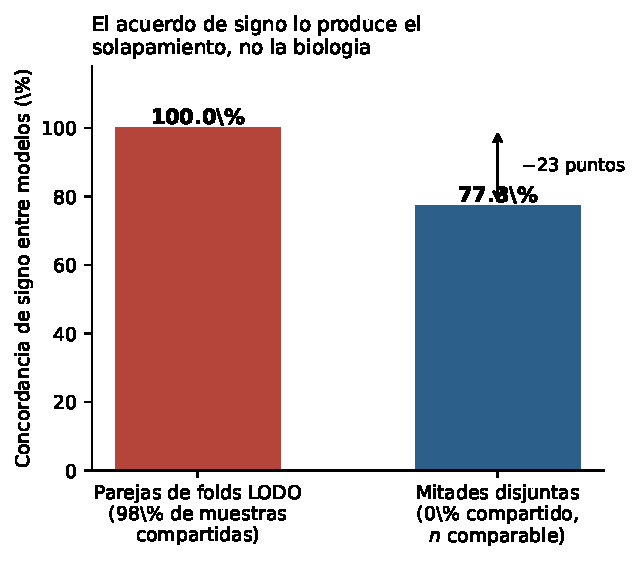
\includegraphics[width=0.58\textwidth]{figuras_auditoria/fig_concordancia_folds.pdf}
\caption[Concordancia de signo y solapamiento]{Concordancia direccional entre
parejas de modelos con entrenamientos de tamaño comparable. La única variable
que cambia entre ambas columnas es la fracción de muestras compartidas.}
\label{fig:falacia}
\end{figure}

La consecuencia sobre la firma previa es directa. De los siete genes destacados
por esta métrica --- SLC6A4, S100A10, KANK3, SH3GL3, HIST1H2BM, ZNF702P y
TOX3 ---, \textbf{ninguno} mantiene coeficiente no nulo y signo constante al
ajustar modelos independientes en las ocho cohortes disjuntas. HIST1H2BM
ilustra el caso con claridad: alcanza un acuerdo de $8/8$ entre \emph{folds}
solapados y no resulta seleccionado en ninguna cohorte individual.

\subsection{Control positivo: clasificación de subtipo histológico}
\label{sec:subtipo}

Los resultados anteriores plantean una pregunta necesaria: si el marco
metodológico no detecta señal reproducible en la tarea tumor frente a sano,
¿está midiendo mal, o simplemente no hay señal que medir? Para distinguir ambas
posibilidades se aplicó el mismo pipeline a una tarea con respuesta conocida y
consecuencia terapéutica real: la distinción entre adenocarcinoma y carcinoma
escamoso, que condiciona la elección de tratamiento --- pemetrexed y
bevacizumab están contraindicados en histología escamosa.

Se emplearon las tres cohortes con histología anotada y ambas clases presentes
(GSE30219, GSE50081 y GSE19188), todas en plataforma GPL570, con 388 muestras y
22\,880 genes comunes. La armonización de códigos requirió atención explícita:
la abreviatura \texttt{SCC} designa carcinoma escamoso en GSE19188 y carcinoma
microcítico en GSE30219, entidades clínicamente opuestas.

\begin{table}[htbp]
\centering
\caption[Control positivo: subtipo histologico]{Validacion LODO de la tarea
adenocarcinoma frente a escamoso sobre las tres cohortes con histologia anotada
y ambas clases presentes (todas en plataforma GPL570).}
\label{tab:subtipo}
\small
\begin{tabular}{lrcrrrr}
\toprule
Cohorte test & $n$ & ADC/Esc. & \emph{Baseline} & Bal.\ acc. & AUC & Ganancia \\
\midrule
GSE30219 & 146 & 85/61 & 0,582 & 0,967 & 0,993 & $+$0,390 \\
GSE50081 & 170 & 127/43 & 0,747 & 0,887 & 0,909 & $+$0,165 \\
GSE19188 & 72 & 45/27 & 0,625 & 0,967 & 0,998 & $+$0,333 \\
\midrule
\multicolumn{4}{l}{\emph{Media}} &
\textbf{0,940} &
\textbf{0,967} &
$+$0,296 \\
\bottomrule
\end{tabular}
\end{table}


El rendimiento es sustancialmente superior al de la tarea tumor frente a sano:
\emph{balanced accuracy} media de \balaccsub{} y AUC media de \aucsub{}, con una ganancia
media de $+$\gananciasub{} sobre el azar informado. Se derivó además una firma de \ngenesfirma{}
genes con $|d|>0{,}8$ y signo concordante en las tres cohortes calculadas de
forma independiente.

La validación más relevante de este resultado no es su magnitud, sino su
contenido. La firma recupera los doce marcadores empleados en inmunohistoquímica
diagnóstica en la práctica clínica, todos en la dirección correcta: siete de
siete para histología escamosa (KRT5, KRT6A, TP63, DSG3, SOX2, PKP1, KRT14) y
cinco de cinco para adenocarcinoma (NAPSA, NKX2-1, SFTPB, SLC34A2, MUC1). Los
primeros puestos del \emph{ranking} --- DSG3, KRT5, CALML3, KRT6B, PKP1, DSC3,
TP63 --- corresponden a desmosomas, queratinas y el programa transcripcional de
TP63, es decir, a linaje celular escamoso y no a composición del tejido.

Este resultado establece que el marco metodológico es capaz de recuperar
biología reproducible cuando existe. Conviene delimitar su alcance: la
distinción entre adenocarcinoma y escamoso está bien caracterizada en la
literatura transcriptómica y su recuperación no constituye un hallazgo nuevo. Su
valor aquí es el de un control positivo, y fue además el análisis que permitió
detectar el desalineamiento descrito en la sección~\ref{sec:auditoria}.

\subsubsection{Límites del clasificador ante histologías no observadas}
\label{sec:dificiles}

El resultado anterior se obtuvo excluyendo \nambiguas{} muestras --- el \pctexcluidas\,\% de los
tumores disponibles --- correspondientes a histologías que no son adenocarcinoma
ni escamoso: neuroendocrino de célula grande, basaloide, carcinoide,
microcítico, célula grande y adenoescamoso. Se excluyeron, por tanto,
precisamente los casos que en la práctica clínica resultan ambiguos. Someter el
modelo a esas muestras es necesario para no sobreestimar su aplicabilidad.

No existe etiqueta correcta que predecir en ellas, de modo que lo evaluado es la
calibración: un modelo prudente debería asignarles probabilidades intermedias.
La métrica fijada de antemano fue el porcentaje de muestras con $P>0{,}9$ o
$P<0{,}1$, y la hipótesis registrada, que superaría el 50\,\%.

\begin{table}[htbp]
\centering
\caption[Histologias excluidas del clasificador de subtipo]{Comportamiento del
clasificador de subtipo ante las histologias que no vio en el entrenamiento
(grupos con $n\geq3$). \emph{Alta conf.} recoge el porcentaje de muestras con
$P>0{,}9$ o $P<0{,}1$, es decir, asignadas con confianza a una categoria a la
que no pertenecen.}
\label{tab:dificiles}
\small
\begin{tabular}{llrrrr}
\toprule
Histologia & Cohorte & $n$ & $P$(esc.) mediana & Alta conf. & A escamoso \\
\midrule
neuroendocrino celula grande & GSE30219 & 56 & 0,161 & 32,1\,\% & 8,9\,\% \\
basaloide & GSE30219 & 39 & 0,927 & 59,0\,\% & 89,7\,\% \\
carcinoide & GSE30219 & 24 & 0,173 & 8,3\,\% & 4,2\,\% \\
microcitico (small cell) & GSE30219 & 21 & 0,272 & 9,5\,\% & 4,8\,\% \\
celula grande & GSE19188 & 19 & 0,409 & 10,5\,\% & 31,6\,\% \\
celula grande & GSE50081 & 7 & 0,236 & 28,6\,\% & 42,9\,\% \\
otro & GSE30219 & 4 & 0,392 & 50,0\,\% & 50,0\,\% \\
celula grande & GSE30219 & 3 & 0,106 & 33,3\,\% & 0,0\,\% \\
\bottomrule
\end{tabular}
\end{table}


\textbf{La hipótesis no se confirmó.} Solo el \pctconfambiguas\,\% de las muestras ambiguas
recibe una asignación de alta confianza, frente al \pctconfvistas\,\% de las muestras que
sí pertenecen a alguna de las dos clases. El modelo es, por tanto, más prudente
ante lo que no ha visto de lo que se había previsto.

El valor agregado oculta, sin embargo, dos comportamientos opuestos que la
figura~\ref{fig:dificiles} separa. El carcinoma basaloide recibe una mediana de
$P(\text{escamoso})=0{,}937$ y se asigna a escamoso en el 89,7\,\% de los casos;
esto no constituye necesariamente un error, dado que varias clasificaciones lo
consideran una variante de carcinoma escamoso, de modo que el modelo puede estar
recuperando la biología correcta. En cambio, de los \nneuro{} tumores neuroendocrinos
(neuroendocrino de célula grande, microcítico y carcinoide), el \pctneuroadc\,\% se asigna
a adenocarcinoma. Este sí es un fallo con consecuencia clínica directa: el
carcinoma microcítico recibe un tratamiento completamente distinto al del cáncer
de pulmón no microcítico, y el modelo lo etiqueta como adenocarcinoma sin
señalar incertidumbre.

\begin{figure}[htbp]
\centering
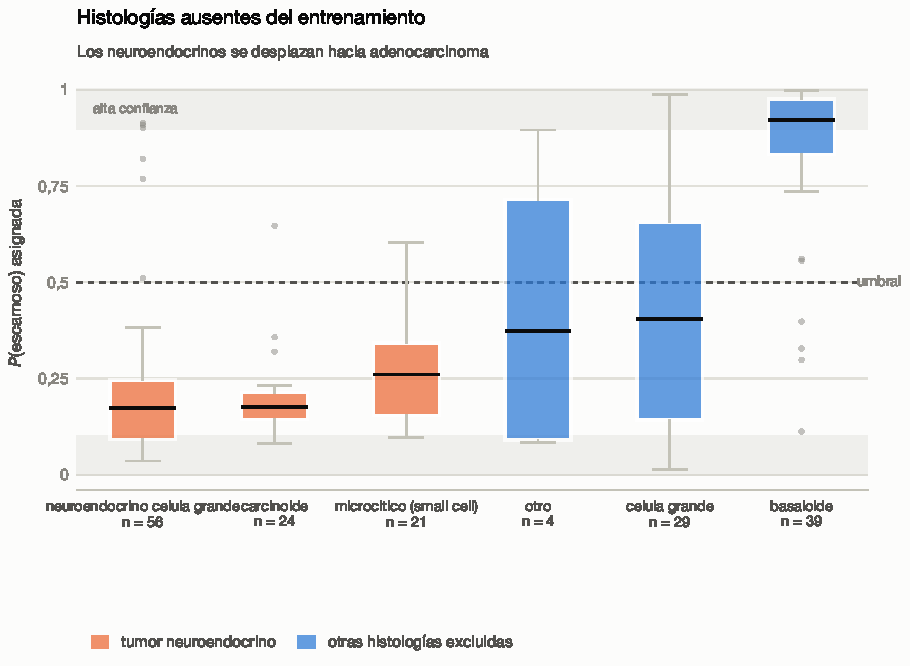
\includegraphics[width=0.95\textwidth]{figuras_auditoria/fig_histologias_excluidas.pdf}
\caption[Histologías excluidas del entrenamiento]{Distribución de la
probabilidad asignada a las histologías ausentes del entrenamiento. En rojo, los
tumores neuroendocrinos, desplazados hacia adenocarcinoma. Las bandas grises
delimitan las regiones de alta confianza.}
\label{fig:dificiles}
\end{figure}

El AUC de \aucsub{} de la sección~\ref{sec:subtipo} es válido únicamente sobre
tumores previamente confirmados como adenocarcinoma o escamoso. El modelo no
puede emplearse como primer filtro sobre un caso sin diagnosticar.

\subsection{Síntesis de resultados}
\label{sec:sintesis}

Los cinco análisis permiten establecer lo siguiente:

\begin{enumerate}
\item Los datos presentan cuatro modos de fallo silencioso y cuantificables:
      tres cohortes declaradas nunca procesadas, \ndesalineadas{} muestras con etiqueta
      cruzada, \sinclasificar{} muestras (\pctsinclasificar\,\%) perdidas en la curación automatizada y
      \nmonoclase{} cohortes de una sola clase empleadas como conjunto de test. Ninguno
      generó un error en tiempo de ejecución.
\item En la tarea tumor frente a sano, la \emph{balanced accuracy} media sobre
      cohortes evaluables es de \balacc{}, con \nosuperan{} de \nev{} por debajo de su propio
      \emph{baseline}.
\item La firma transfiere su capacidad de ordenación entre cohortes (AUC medio
      \aucmedia{}) pero no su umbral de decisión (especificidad media \especmedia{}), un
      problema de calibración inducido por el desbalance del entrenamiento.
\item La composición tisular explica una parte sustancial de la señal
      ($\rho=-\rhotumoresabs$ entre tumores) sin agotarla, y coexiste con un eje de
      proliferación no previsto.
\item La consistencia de signo entre \emph{folds} LODO no mide reproducibilidad
      biológica: alcanza el \conclodo\,\% frente al \concdisjunta\,\% de modelos disjuntos
      comparables, y ninguno de los siete genes destacados por esa métrica
      replica de forma independiente.
\item El marco metodológico sí recupera biología reproducible cuando existe
      (subtipo histológico, AUC \aucsub{}, con los doce marcadores de
      inmunohistoquímica recuperados), con la limitación de no reconocer las
      histologías ausentes del entrenamiento.
\end{enumerate}

%   % =====================================================================
% CAPITULO 6 - DISCUSION
% Sustituye al capitulo 6 de la version anterior de la memoria.
% =====================================================================

\section{Discusión}
\label{cap:discusion}

\subsection{Reorientación del objeto de estudio}
\label{sec:disc-reorientacion}

El planteamiento inicial de este trabajo perseguía identificar biomarcadores
transcriptómicos universales de cáncer de pulmón mediante la integración de
múltiples cohortes públicas. Los resultados del capítulo anterior no sostienen
ese objetivo, y conviene ser explícito sobre por qué.

La firma derivada del contraste entre tejido tumoral y tejido sano adyacente
reúne tres características que impiden interpretarla como un conjunto de
biomarcadores: su señal procede en parte sustancial de la composición del tejido
más que de biología tumoral específica (sección~\ref{sec:composicion}); su
estabilidad aparente era un artefacto del diseño de validación
(sección~\ref{sec:falacia}); y la tarea que resuelve no constituye un problema
clínico, dado que la distinción entre tumor y parénquima normal la resuelve el
examen histopatológico convencional con fiabilidad superior, coste
incomparablemente menor y sobre la misma muestra ya disponible.

Esto no invalida el framework desarrollado. Lo que invalida es la lectura que se
había hecho de sus resultados. El pipeline descarga, normaliza, curó
metadatos mediante modelos de lenguaje, ejecuta análisis diferencial, entrena
modelos y valida de forma externa; todos esos componentes funcionan, y el
control positivo de la sección~\ref{sec:subtipo} demuestra que recuperan biología
reproducible cuando está presente. La contribución defendible de este trabajo no
es, por tanto, una firma molecular, sino la caracterización sistemática de los
modos en que estos pipelines fallan sin avisar, y un conjunto de controles
concretos para detectarlos.

\subsection{Los cuatro modos de fallo silencioso}
\label{sec:disc-fallos}

Los problemas documentados en la sección~\ref{sec:auditoria} comparten un rasgo
que los hace especialmente peligrosos: ninguno interrumpe la ejecución. El
pipeline termina, escribe sus ficheros y produce tablas de aspecto correcto.

\paragraph{El desalineamiento como fallo indistinguible.} El caso de GSE30219 es
instructivo porque su efecto imita exactamente el de una hipótesis nula
verdadera. Un AUC de 0,56 sobre una cohorte de 146 tumores es perfectamente
compatible con la conclusión «esta señal no generaliza a esta cohorte», y ese es
el tipo de resultado que un trabajo honesto acepta y reporta. Solo la
comparación con marcadores de referencia externos --- la observación de que KRT5
mostraba una diferencia de $+0{,}90$ en esta cohorte frente a $+5{,}32$ y
$+5{,}66$ en las otras dos --- reveló que la señal estaba presente pero
desacoplada de las etiquetas. La lección metodológica es que la validación
frente a conocimiento biológico previo no es un adorno interpretativo, sino un
control de integridad de los datos.

Resulta pertinente señalar que el análisis original no se vio afectado por este
error, y la razón es instructiva: GSE30219 contiene una sola clase, de modo que
intercambiar etiquetas idénticas entre sí no altera nada. El fallo permaneció
latente y solo se manifestó al plantear una pregunta que utilizara la
información clínica. Un pipeline puede arrastrar errores de este tipo durante
todo su ciclo de vida sin que se manifiesten, hasta que alguien formula la
pregunta adecuada.

\paragraph{La curación automatizada como fuente de sesgo de selección.} El
empleo de modelos de lenguaje para homogeneizar metadatos clínicos heterogéneos
es una de las aportaciones metodológicamente más interesantes del framework, y
su comportamiento bimodal --- éxito prácticamente completo en ocho cohortes,
colapso en dos --- merece una lectura cuidadosa. El problema no es la tasa
global del 82,8\,\%, sino que las pérdidas no son aleatorias: se concentran en
cohortes concretas y, dentro de ellas, afectan a la práctica totalidad de las
muestras. GSE40791 pasó de 194 muestras a 12, y las 12 supervivientes presentan
una composición de clases (10 controles y 2 tumores) que no representa al
estudio original. El resultado es un sesgo de selección introducido por una capa
de procesamiento automático, no declarado como tal en ningún punto del
pipeline. La recomendación que se deriva es que cualquier etapa de curación
automatizada debe reportar su tasa de éxito por cohorte como parte de los
resultados, y que las cohortes con tasas bajas deben excluirse explícitamente en
lugar de participar con su fracción superviviente.

\paragraph{Cohortes de una sola clase.} Que GSE30219 y GSE50081 no contengan
controles no es un defecto de esas cohortes: son estudios de supervivencia,
diseñados para correlacionar expresión con evolución clínica, y su composición es
la correcta para su propósito. El error consiste en emplearlas como conjunto de
test de un clasificador binario. Este fallo es además el más fácil de detectar
automáticamente --- basta comprobar el número de clases presentes antes de
evaluar --- y el más fácil de pasar por alto cuando la métrica reportada es
únicamente la \emph{accuracy}, porque produce precisamente los valores más altos
de la tabla.

\subsection{Discriminación y decisión como propiedades independientes}
\label{sec:disc-calibracion}

El hallazgo de la sección~\ref{sec:calibracion} no estaba previsto y es, a
nuestro juicio, el resultado de mayor utilidad práctica del trabajo. La
coexistencia de un AUC medio de 0,925 con una \emph{balanced accuracy} media de
0,773, y su expresión extrema en GSE40791 (\emph{accuracy} 0,167 con AUC 1,000),
descompone lo que habitualmente se trata como un único atributo --- «el modelo
generaliza» o «no generaliza» --- en dos propiedades que transfieren de forma
independiente entre cohortes.

La capacidad de ordenación transfiere bien: la firma sitúa consistentemente las
muestras tumorales por encima de los controles en cohortes que nunca ha visto. El
umbral de decisión no transfiere: el punto de corte aprendido sobre una
distribución de clases determinada (938 tumores frente a 219 controles) deja de
ser adecuado cuando la cohorte de destino presenta otra composición. La
sensibilidad media de 0,983 frente a una especificidad media de 0,563 describe un
modelo que ha aprendido, razonablemente dada su dieta de entrenamiento, que
predecir «tumor» casi siempre acierta.

Esta lectura reinterpreta un patrón que el análisis original registraba sin
explicar. Los casos de \emph{accuracy} próxima a 0,5 acompañada de AUC próximo a
1,0 se habían atribuido a la dificultad intrínseca del problema, al tamaño
muestral reducido o a particularidades técnicas de los estudios. No era ninguna
de esas cosas: era un problema de calibración, y los problemas de calibración
son corregibles. La vía inmediata es la ponderación de clases en el
entrenamiento; la más robusta, reportar métricas independientes del umbral (AUC,
precisión media) junto con métricas de decisión, y ajustar el punto de corte
sobre la cohorte de destino cuando el escenario de aplicación lo permita.

\subsection{Qué mide la firma: composición, proliferación y biología}
\label{sec:disc-composicion}

La hipótesis de que la firma tumor frente a sano capturase esencialmente
composición tisular no se confirmó al umbral fijado de antemano
($|\rho|>0{,}7$; obtenido $\rho=-0{,}637$). Mantener ese criterio obliga a una
conclusión más matizada, y probablemente más correcta, que la hipótesis de
partida.

La composición tisular explica una fracción sustancial de la señal. La evidencia
es convergente: la correlación entre el \emph{score} del clasificador y el
contenido de pulmón normal persiste al restringir el análisis a muestras
tumorales, alcanzando $\rho=-0{,}870$ ($p=7\times10^{-71}$) en la cohorte con
mayor número de tumores evaluables; y cinco de los cincuenta genes principales de
la firma son marcadores canónicos de epitelio alveolar y estroma pulmonar normal,
con $\log$FC en torno a $-4$. Interpretados como biomarcadores tumorales, genes
como AGER, CLDN18 o SFTPC informan principalmente de cuánto parénquima sano
conserva la muestra.

Pero no la agotan. El segundo eje detectado --- correlación positiva con
proliferación, entre $+0{,}267$ y $+0{,}719$ --- indica que el clasificador
integra al menos dos fenómenos distintos, y el segundo sí es biología tumoral en
sentido estricto. La descripción más ajustada de lo que mide la firma es
«pérdida de arquitectura alvéolo-capilar normal más ganancia de actividad
proliferativa», una combinación real, reproducible y de escaso valor
discriminativo por ser común a la práctica totalidad de los tumores sólidos.

Debe señalarse una limitación de este análisis: solo cuatro cohortes reunían
tumores suficientes ($n\geq8$) para el contraste restringido, y los estimadores
presentan heterogeneidad notable entre ellas ($\rho$ de $-0{,}343$ a
$-0{,}870$). Un abordaje más riguroso emplearía métodos de deconvolución celular
para estimar la proporción de cada tipo celular, en lugar de un panel de
marcadores promediado.

\subsection{Implicaciones sobre el diseño de la validación externa}
\label{sec:disc-lodo}

La estrategia LODO es metodológicamente superior a la validación cruzada
convencional dentro de un mismo estudio, y su adopción sigue siendo escasa en la
literatura de biomarcadores transcriptómicos. Este trabajo no cuestiona esa
elección, sino dos usos concretos que se hicieron de ella.

El primero es de terminología con consecuencias conceptuales: LODO no corrige el
efecto lote, lo \emph{mide}. Presentarla como mecanismo de superación del
\emph{batch effect} confunde la naturaleza del procedimiento. En el pipeline
analizado no existe corrección de lote alguna --- solo normalización por
cuantiles dentro de cada estudio y estandarización por estudio ---, y la
degradación de rendimiento entre cohortes que LODO revela \emph{es} la magnitud
del problema, no su solución.

El segundo es el uso de los \emph{folds} LODO como réplicas para medir
estabilidad. La demostración de la sección~\ref{sec:falacia} es cuantitativa y,
en nuestra opinión, generalizable más allá de este trabajo: cuando el número de
cohortes es moderado, los conjuntos de entrenamiento de los distintos
\emph{folds} comparten una mediana del 97,6\,\% de sus muestras, y la
concordancia direccional resultante es del 100,0\,\% en la totalidad de los
pares. Una métrica cuyo valor está determinado por el diseño no puede aportar
evidencia sobre el fenómeno estudiado. El control con mitades disjuntas de
tamaño comparable (73,98\,\%) delimita cuánto de ese 100\,\% procede del
solapamiento.

La consecuencia sobre los siete genes previamente destacados es contundente:
ninguno replica al ajustar modelos independientes. Esto no significa que carezcan
de interés biológico --- SLC6A4 y KANK3 son marcadores endoteliales pulmonares
bien caracterizados, coherentes con la interpretación composicional de la
sección anterior ---, sino que la evidencia aportada para priorizarlos no era
evidencia. La alternativa empleada en la sección~\ref{sec:subtipo}, exigir
concordancia de tamaño de efecto en cohortes ajustadas por separado, es más
exigente y produjo una firma que recupera marcadores de uso clínico establecido.

\subsection{Alcance y limitaciones del control positivo}
\label{sec:disc-subtipo}

La clasificación de subtipo histológico cumple su función como control positivo:
demuestra que el marco metodológico detecta biología reproducible cuando existe,
con AUC medio de 0,967 y recuperación completa de los doce marcadores de
inmunohistoquímica diagnóstica. Conviene, no obstante, precisar tres límites.

Primero, la distinción entre adenocarcinoma y carcinoma escamoso está
extensamente caracterizada en transcriptómica y su recuperación no constituye una
aportación original. Su valor es de verificación, no de descubrimiento.

Segundo, el resultado se obtuvo excluyendo el 31,3\,\% de los tumores
disponibles, precisamente los de histología ambigua. El análisis de la
sección~\ref{sec:dificiles} muestra que el modelo es más prudente ante esas
muestras de lo previsto (29,9\,\% de asignaciones de alta confianza frente al
62,6\,\% en muestras de clase conocida; la hipótesis registrada no se confirmó),
pero también que el 93\,\% de los 101 tumores neuroendocrinos se etiqueta como
adenocarcinoma. Dado que el carcinoma microcítico requiere un abordaje
terapéutico completamente distinto, esta es una limitación con consecuencia
clínica y no meramente estadística.

Tercero, las tres cohortes comparten plataforma (GPL570), de modo que el
resultado no informa sobre transferencia entre tecnologías de medición. Las tres
cohortes de RNA-seq que habrían permitido evaluarlo son precisamente las que el
pipeline no llegó a procesar.

\subsection{Recomendaciones metodológicas}
\label{sec:disc-recomendaciones}

De los resultados obtenidos se derivan seis controles concretos, aplicables a
cualquier pipeline de descubrimiento de biomarcadores sobre repositorios
públicos:

\begin{enumerate}
\item \textbf{Alinear muestras y metadatos por identificador explícito}, nunca
      por posición, y verificar la correspondencia como paso previo a cualquier
      análisis. La coincidencia de longitudes no implica coincidencia de orden.
\item \textbf{Validar contra marcadores biológicos conocidos} antes de
      interpretar cualquier resultado. Un panel de referencia de la patología
      estudiada funciona como control de integridad de los datos y detecta
      fallos que ninguna comprobación de formato revela.
\item \textbf{Reportar el \emph{baseline} de clase mayoritaria} junto a toda
      métrica de rendimiento, y excluir explícitamente las cohortes de una sola
      clase de la evaluación, indicándolo en las tablas.
\item \textbf{Separar métricas de discriminación y de decisión.} Informar AUC y
      \emph{balanced accuracy} conjuntamente, con sensibilidad y especificidad
      desglosadas; su divergencia identifica problemas de calibración que la
      \emph{accuracy} agregada oculta.
\item \textbf{Medir la estabilidad sobre particiones disjuntas}, no sobre
      \emph{folds} solapados, y declarar la fracción de muestras compartidas
      cuando se empleen estas últimas.
\item \textbf{Cuantificar y reportar la tasa de éxito de toda etapa de curación
      automatizada} por cohorte, tratando las pérdidas elevadas como criterio de
      exclusión y no como merma silenciosa del tamaño muestral.
\end{enumerate}

\subsection{Líneas futuras}
\label{sec:disc-futuro}

Los datos ya descargados permiten abordar preguntas que este trabajo no ha
explorado y que resultan más informativas que la comparación entre tumor y tejido
sano. GSE30219 y GSE50081 disponen de seguimiento clínico completo (307 y 181
tumores, con 200 y 75 eventos de mortalidad respectivamente), lo que habilita
análisis de supervivencia con validación cruzada entre cohortes. GSE31210
incluye el estado de los principales genes conductores --- 127 tumores con
mutación de EGFR, 20 de KRAS, 11 con fusión de ALK y 68 sin ninguna de las tres
alteraciones ---, lo que permite plantear la predicción de alteración
conductora a partir del perfil de expresión. Ambas son preguntas cuya respuesta
no se conoce de antemano por inspección de la muestra, condición que la tarea
tumor frente a sano no cumplía.

En el plano metodológico, tres extensiones mejorarían el rigor de los análisis
presentados: el empleo de deconvolución celular en lugar de paneles de
marcadores promediados para cuantificar composición tisular; la incorporación de
corrección de lote explícita, con evaluación de su efecto sobre la transferencia
entre cohortes; y la recuperación de las tres cohortes de RNA-seq no procesadas,
que permitirían por primera vez evaluar la generalización entre plataformas de
medición distintas.

% en el punto correspondiente del documento principal, y copiar las
% carpetas figuras_auditoria/ y tablas_auditoria/ junto al .tex.
% =====================================================================

\documentclass[11pt,a4paper]{article}

\usepackage[utf8]{inputenc}
\usepackage[T1]{fontenc}
\usepackage{lmodern}       % fuente escalable: microtype requiere Type1, no bitmap
\usepackage[spanish,es-tabla,es-noquoting]{babel}
\usepackage[a4paper,margin=2.6cm]{geometry}
\usepackage{booktabs}
\usepackage{multirow}
\usepackage{graphicx}
\usepackage{caption}
\usepackage{amsmath}
\usepackage{amssymb}
\usepackage{enumitem}
\usepackage[expansion=false]{microtype}
\usepackage[hidelinks]{hyperref}

% Cifras generadas desde los CSV de resultados (generar_tablas_latex.py).
% La prosa de los capitulos las usa como macros, de modo que no puede citar
% un numero que los analisis no contengan.
% Generado por agentes/generar_tablas_latex.py. No editar a mano.
% Cada macro procede de un CSV de resultados: la prosa de la memoria
% no puede citar una cifra que los analisis no contengan.

\newcommand{\balacc}{0,772}
\newcommand{\aucmedia}{0,925}
\newcommand{\sensmedia}{0,983}
\newcommand{\especmedia}{0,561}
\newcommand{\basemedia}{0,609}
\newcommand{\gananciamedia}{0,115}
\newcommand{\accundece}{0,778}
\newcommand{\nev}{8}
\newcommand{\ncohortes}{11}
\newcommand{\nosuperan}{3}
\newcommand{\nmuestras}{1397}
\newcommand{\sinclasificar}{240}
\newcommand{\pctsinclasificar}{17,2}
\newcommand{\ndesalineadas}{307}
\newcommand{\nmonoclase}{3}
\newcommand{\rhotumores}{-0,626}
\newcommand{\rhotumoresabs}{0,626}
\newcommand{\nrho}{4}
\newcommand{\nrhosupera}{2}
\newcommand{\rhomax}{-0,858}
\newcommand{\rhoprolifmin}{0,314}
\newcommand{\rhoprolifmax}{0,667}
\newcommand{\conclodo}{100,0}
\newcommand{\concdisjunta}{77,33}
\newcommand{\caidaconc}{23}
\newcommand{\genesfolds}{12}
\newcommand{\genesdisjuntas}{0}
\newcommand{\balaccsub}{0,940}
\newcommand{\aucsub}{0,968}
\newcommand{\gananciasub}{0,296}
\newcommand{\nsub}{388}
\newcommand{\nambiguas}{177}
\newcommand{\pctexcluidas}{31,3}
\newcommand{\pctconfambiguas}{29,4}
\newcommand{\pctconfvistas}{63,1}
\newcommand{\nneuro}{101}
\newcommand{\pctneuroadc}{92}
\newcommand{\accaa}{0,500}
\newcommand{\baseaa}{0,500}
\newcommand{\accbb}{0,894}
\newcommand{\basebb}{0,919}
\newcommand{\acccc}{0,167}
\newcommand{\basecc}{0,833}
\newcommand{\ngenesfirma}{1174}


\captionsetup{font=small,labelfont=bf}
\setlength{\parskip}{0.4em}

\title{\textbf{Capítulos 5 y 6 (versión revisada)}\\[0.3em]
\large Framework transcriptómico para la auditoría de reproducibilidad\\
de firmas de expresión en cáncer de pulmón}
\author{Daniel Tapia Díez}
\date{Versión de trabajo generada automáticamente desde los resultados}

\begin{document}
\maketitle

\begin{abstract}
\noindent Documento de trabajo con los capítulos de Resultados y Discusión
reescritos a partir de los análisis de los pasos 14 a 18. Todas las tablas se
generan mediante \texttt{agentes/generar\_tablas\_latex.py} y todas las figuras
mediante \texttt{agentes/generar\_figuras\_auditoria.py}, en ambos casos
directamente desde los ficheros CSV de resultados, de modo que ningún valor
numérico está transcrito a mano y una reejecución de los análisis actualiza el
documento de forma consistente.

\medskip
\noindent De las cinco hipótesis contrastadas, tres se confirmaron y dos no. Las
dos que no se confirmaron se mantienen con el umbral fijado antes de ejecutar el
análisis y se reportan como resultaron.
\end{abstract}

\tableofcontents
\bigskip

% =====================================================================
% CAPITULO 5 - RESULTADOS
% Sustituye al capitulo 5 de la version anterior de la memoria.
% Las tablas se generan con agentes/generar_tablas_latex.py y las figuras
% con agentes/generar_figuras_auditoria.py, ambas a partir de los CSV de
% los pasos 14-18. Ningun valor esta escrito a mano en este fichero salvo
% los citados en el texto corrido.
% =====================================================================

\section{Resultados}
\label{cap:resultados}

Este capítulo se organiza en torno a una distinción que resultó determinante:
la diferencia entre \emph{lo que un modelo consigue} y \emph{lo que una métrica
parece indicar}. Los cinco análisis que se presentan fueron especificados con su
hipótesis y su umbral de decisión fijados antes de ejecutarse. Dos de las cinco
hipótesis no se confirmaron, y se reportan como resultaron; mantener el criterio
original en esos dos casos es parte del resultado, no una concesión.

\subsection{Auditoría de integridad de las cohortes}
\label{sec:auditoria}

Antes de reevaluar cualquier modelo se auditó el estado real de los datos sobre
los que se construyeron los análisis. La tabla~\ref{tab:auditoria} resume las
once cohortes con datos procesados.

\begin{table}[htbp]
\centering
\caption[Auditoria de integridad de las cohortes]{Auditoria de integridad de
las once cohortes con datos procesados. La columna \emph{Desalin.} indica
muestras cuya etiqueta clinica corresponde a otro paciente por asignacion
posicional; \emph{Eval.} indica si la cohorte contiene ambas clases y por
tanto es evaluable como conjunto de test.}
\label{tab:auditoria}
\small
\begin{tabular}{llrrrrrcc}
\toprule
Cohorte & Plataforma & $n$ & Sanas & Enfermas & Sin clas. & Curacion & Desalin. & Eval. \\
\midrule
GSE118370 & GPL570 & 12 & 6 & 6 & 0 & 100,0\,\% & OK & si \\
GSE140797 & GPL13497 & 14 & 0 & 7 & 7 & 50,0\,\% & OK & \textbf{no} \\
GSE18842 & GPL570 & 91 & 45 & 46 & 0 & 100,0\,\% & OK & si \\
GSE19188 & GPL570 & 156 & 65 & 91 & 0 & 100,0\,\% & OK & si \\
GSE19804 & GPL570 & 120 & 60 & 60 & 0 & 100,0\,\% & OK & si \\
GSE23066 & GPL570 & 10 & 5 & 5 & 0 & 100,0\,\% & OK & si \\
GSE30219 & GPL570 & 307 & 0 & 307 & 0 & 100,0\,\% & \textbf{307/307} & \textbf{no} \\
GSE31210 & GPL570 & 246 & 20 & 226 & 0 & 100,0\,\% & OK & si \\
GSE40791 & GPL570 & 194 & 10 & 2 & 182 & 6,2\,\% & OK & si \\
GSE50081 & GPL570 & 181 & 0 & 181 & 0 & 100,0\,\% & OK & \textbf{no} \\
GSE7670 & GPL96 & 66 & 8 & 7 & 51 & 22,7\,\% & OK & si \\
\midrule
\textbf{Total} & & \textbf{1397} & 219 &
938 & \textbf{240} &
\textbf{82,8\,\%} & 307 & 8/11 \\
\bottomrule
\end{tabular}
\end{table}


La auditoría reveló cuatro problemas de naturaleza distinta.

\paragraph{Cobertura incompleta y silenciosa.} De las doce cohortes declaradas
en \texttt{datasets.txt}, tres nunca llegaron a procesarse: GSE40419, GSE81089 y
GSE140343, precisamente las tres basadas en RNA-seq. El fallo no generó ningún
error: el pipeline continuó y produjo resultados aparentemente completos. En
sentido inverso, dos cohortes presentes en los resultados (GSE118370 y
GSE140797) no figuran en el fichero de declaración. La cohorte efectivamente
analizada no coincide, por tanto, con la cohorte declarada.

\paragraph{Desalineamiento entre muestras y etiquetas clínicas.} En GSE30219,
las 307 columnas de la matriz de expresión están ordenadas de forma distinta a
las filas del fichero de metadatos, aunque ambos contengan el mismo conjunto de
muestras. Asignar las etiquetas por posición --- operación habitual cuando las
longitudes coinciden --- adjudica a cada muestra la información clínica de otro
paciente. El error afecta a la totalidad de la cohorte y no produce ninguna
señal de aviso.

Su efecto práctico se cuantificó de forma directa. Al entrenar el clasificador
de subtipo histológico (sección~\ref{sec:subtipo}) sobre los datos desalineados,
el AUC obtenido sobre esta cohorte fue de 0,56, indistinguible del azar. Con el
alineamiento corregido mediante identificador de muestra, el mismo modelo y los
mismos datos alcanzaron un AUC de 0,99. El desalineamiento no degrada el
resultado: lo destruye por completo, y lo hace de forma indistinguible de una
ausencia genuina de señal biológica.

\paragraph{Fallo parcial de la curación clínica automatizada.} La asignación de
etiquetas mediante modelo de lenguaje funcionó de forma completa en ocho de las
once cohortes, pero falló de manera severa en dos: en GSE40791 dejó sin
clasificar 182 de 194 muestras (93,8\,\%) y en GSE7670, 51 de 66 (77,3\,\%). En
conjunto, \sinclasificar{} de las \nmuestras{} muestras disponibles (\pctsinclasificar\,\%) quedaron fuera del
análisis por esta vía. La figura~\ref{fig:curacion} muestra la distribución por
cohorte. El patrón es relevante: el fallo no es gradual sino bimodal --- la
curación funciona casi perfectamente o se colapsa --- lo que sugiere
sensibilidad al formato concreto de los metadatos más que una limitación
uniforme de la capacidad del modelo.

\begin{figure}[htbp]
\centering
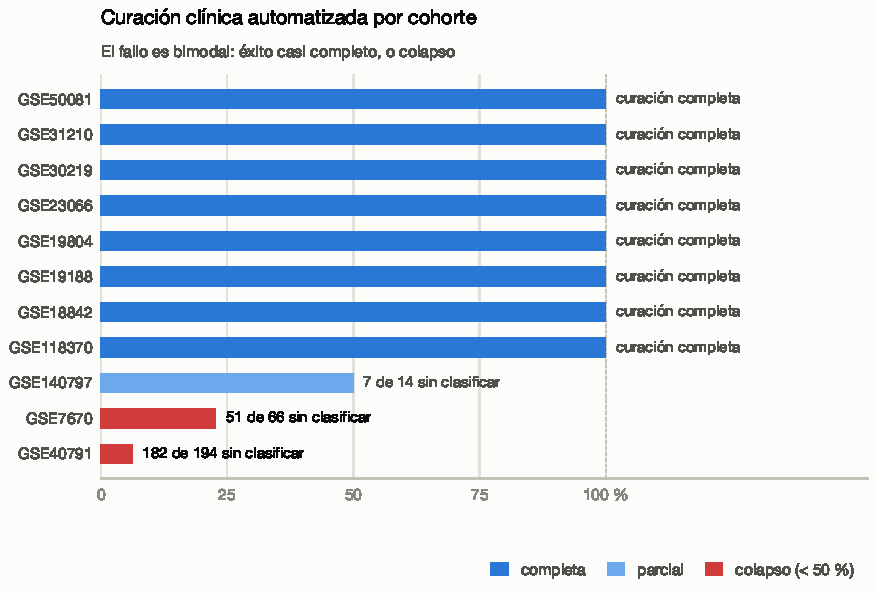
\includegraphics[width=0.95\textwidth]{figuras_auditoria/fig_curacion_llm.pdf}
\caption[Tasa de éxito de la curación automatizada]{Proporción de muestras a las
que la curación mediante modelo de lenguaje asignó una etiqueta utilizable. El
comportamiento es bimodal: éxito casi completo o colapso.}
\label{fig:curacion}
\end{figure}

\paragraph{Cohortes no evaluables empleadas como conjunto de test.} Tres
cohortes contienen únicamente muestras tumorales y ningún control: GSE30219
(307 muestras), GSE50081 (181) y GSE140797 (7). Una cohorte de una sola clase
puede formar parte legítimamente del conjunto de entrenamiento, pero no puede
funcionar como conjunto de test: en ella, la estrategia trivial de predecir
siempre la clase presente alcanza por definición una \emph{accuracy} de 1,000.
Cualquier valor elevado obtenido sobre estas cohortes es una consecuencia
aritmética de su composición, no una medida de capacidad predictiva.

\subsection{Reevaluación de la validación LODO}
\label{sec:lodo}

Se repitió la validación \emph{Leave-One-Dataset-Out} sobre la tarea tumor
frente a sano conservando deliberadamente el modelo original (regresión
logística con penalización $L_1$, $C=0{,}5$, sin ponderación de clases). Solo se
modificaron dos elementos: el alineamiento muestra--etiqueta y el conjunto de
métricas reportadas. Aislar así las variables permite atribuir cualquier
diferencia observada al modo de medir, y no a un cambio de método.

La hipótesis registrada fue que el rendimiento medio descendería respecto al
valor previamente reportado y que GSE31210 y GSE40791 quedarían por debajo de su
propio \emph{baseline}. La tabla~\ref{tab:lodo-honesto} recoge el resultado.

\begin{table}[htbp]
\centering
\caption[Validacion LODO con metricas completas]{Validacion LODO de la tarea
tumor frente a sano, con el mismo modelo del analisis original (LASSO, $C=0{,}5$)
y el alineamiento muestra--etiqueta corregido. Se anaden el \emph{baseline} de
clase mayoritaria y la \emph{balanced accuracy}; las tres cohortes con una sola
clase se marcan como no evaluables. En negrita, las cohortes que no superan su
propio \emph{baseline}.}
\label{tab:lodo-honesto}
\small
\begin{tabular}{lrcrrrrrr}
\toprule
Cohorte test & $n$ & Sano/Enf. & \emph{Baseline} & Acc. & Bal.\ acc. & AUC & Sens. & Espec. \\
\midrule
GSE118370 & 12 & 6/6 & 0,500 & 0,917 & 0,917 & 1,000 & 1,000 & 0,833 \\
GSE18842 & 91 & 45/46 & 0,505 & 0,890 & 0,889 & 1,000 & 1,000 & 0,778 \\
GSE19188 & 156 & 65/91 & 0,583 & 0,923 & 0,912 & 0,984 & 0,978 & 0,846 \\
GSE19804 & 120 & 60/60 & 0,500 & 0,775 & 0,775 & 0,984 & 1,000 & 0,550 \\
GSE7670 & 15 & 8/7 & 0,533 & 0,733 & 0,750 & 1,000 & 1,000 & 0,500 \\
GSE23066 & 10 & 5/5 & 0,500 & 0,500 & 0,500 & 0,440 & 1,000 & 0,000 \\
GSE31210 & 246 & 20/226 & 0,919 & 0,898 & 0,945 & 0,993 & 0,889 & 1,000 \\
GSE40791 & 12 & 10/2 & 0,833 & 0,167 & 0,500 & 1,000 & 1,000 & 0,000 \\
GSE50081 & 181 & 0/181 & 1,000 & 0,967 & \multicolumn{4}{c}{\emph{no evaluable: una sola clase}} \\
GSE30219 & 307 & 0/307 & 1,000 & 0,941 & \multicolumn{4}{c}{\emph{no evaluable: una sola clase}} \\
GSE140797 & 7 & 0/7 & 1,000 & 0,857 & \multicolumn{4}{c}{\emph{no evaluable: una sola clase}} \\
\midrule
\multicolumn{5}{l}{\emph{Media sobre las 8 cohortes evaluables}} &
\textbf{0,773} &
\textbf{0,925} &
0,983 & 0,563 \\
\multicolumn{5}{l}{\emph{Media de \emph{accuracy} sobre las 11 (como en el analisis original)}} &
\multicolumn{4}{c}{0,779} \\
\bottomrule
\end{tabular}
\end{table}


La hipótesis se confirmó. Sobre las ocho cohortes evaluables, la
\emph{balanced accuracy} media fue de \balacc{} y la ganancia media respecto al azar
informado, de $+$\gananciamedia{}. \nosuperan{} de las \nev{} cohortes evaluables no superan su
propio \emph{baseline}: GSE23066 lo iguala (\accaa{} frente a \baseaa{}), GSE31210
queda ligeramente por debajo (\accbb{} frente a \basebb{}) y GSE40791 lo hace de forma
drástica (\acccc{} frente a \basecc{}). La figura~\ref{fig:lodo} representa cada
cohorte frente a su umbral trivial.

\begin{figure}[htbp]
\centering
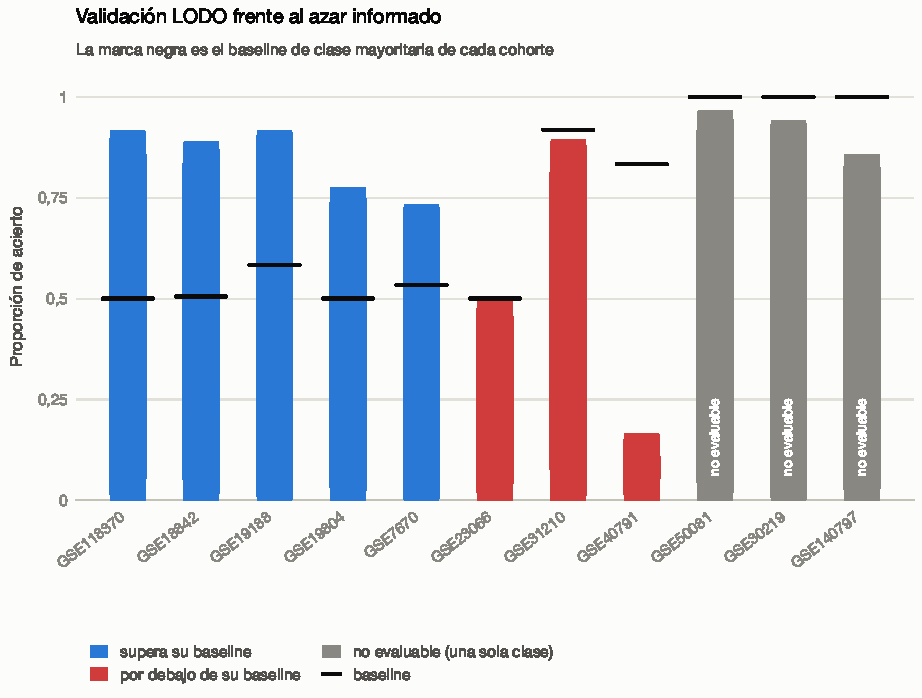
\includegraphics[width=\textwidth]{figuras_auditoria/fig_lodo_vs_baseline.pdf}
\caption[Validación LODO frente al azar informado]{\emph{Accuracy} obtenida en
cada cohorte externa (barras) frente al \emph{baseline} de clase mayoritaria
(marcas horizontales). En rojo, las cohortes evaluables que no superan su
umbral trivial; en gris, las tres cohortes de una sola clase, donde la métrica
carece de contenido.}
\label{fig:lodo}
\end{figure}

\subsubsection{Un hallazgo no previsto: discriminación sin decisión}
\label{sec:calibracion}

El análisis produjo un resultado que no formaba parte de la hipótesis registrada
y que resultó ser el más informativo del capítulo. Sobre las mismas ocho
cohortes evaluables, el AUC medio fue de \aucmedia{} mientras que la
\emph{balanced accuracy} media se quedó en \balacc{}. La divergencia entre ambas
métricas es sistemática, no anecdótica, y alcanza su expresión más extrema en
GSE40791: \emph{accuracy} de \acccc{} con un AUC de 1,000.

Un AUC de 1,000 indica que el modelo ordena perfectamente las muestras: existe
un umbral que las separa sin error. Una \emph{accuracy} de 0,167 indica que el
umbral empleado --- el valor por defecto de 0,5 --- no es ese. Las columnas de
sensibilidad y especificidad de la tabla~\ref{tab:lodo-honesto} identifican la
causa: la sensibilidad media es de \sensmedia{} y la especificidad media, de \especmedia{}. El
modelo clasifica como tumoral casi todo lo que recibe. Ese sesgo es coherente
con la composición del conjunto de entrenamiento, que reúne 938 muestras
tumorales frente a 219 controles.

La conclusión es que la firma transcriptómica sí transfiere entre cohortes
independientes en cuanto a su \emph{capacidad de ordenación}, pero el
\emph{punto de corte} no transfiere. La figura~\ref{fig:auc} representa ambas
dimensiones. Esta distinción tiene una consecuencia metodológica inmediata: los
valores de \emph{accuracy} próximos a 0,5 acompañados de un AUC próximo a 1,0
que aparecían en el análisis original no eran ruido ni indicios de dificultad
intrínseca del problema, sino la manifestación de un problema de calibración
enteramente corregible.

\begin{figure}[htbp]
\centering
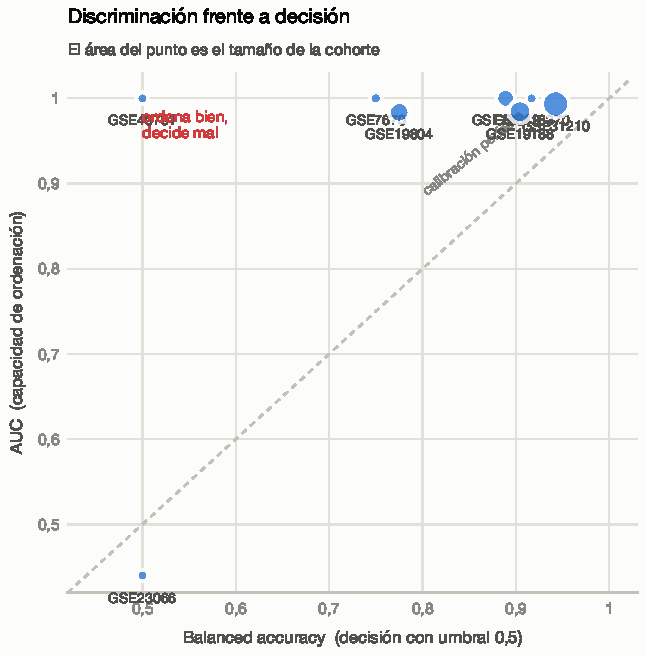
\includegraphics[width=0.62\textwidth]{figuras_auditoria/fig_auc_vs_balacc.pdf}
\caption[Discriminación frente a decisión]{Cada punto es una cohorte externa; el
tamaño es proporcional al número de muestras. La distancia a la diagonal mide
cuánto se pierde por un umbral de decisión mal calibrado. Las cohortes situadas
arriba a la izquierda ordenan bien y deciden mal.}
\label{fig:auc}
\end{figure}

\subsection{Naturaleza de la señal: composición tisular frente a biología tumoral}
\label{sec:composicion}

Los genes que encabezaban la firma de consenso previa sugerían una
interpretación alternativa a la de biomarcadores tumorales. Entre los cincuenta
primeros aparecen cinco marcadores canónicos de tejido pulmonar sano --- AGER y
CLDN18 (epitelio alveolar tipo~I), SFTPC (tipo~II), FABP4 y WIF1 --- todos con
un $\log$FC medio próximo a $-4$, junto con COL10A1, característico de estroma
desmoplásico, al alza. Ese perfil describe la sustitución de parénquima pulmonar
normal por tejido tumoral y estroma reactivo, es decir, una diferencia de
\emph{composición} de la muestra.

Para contrastarlo se construyó un \emph{score} de contenido de pulmón normal a
partir de un panel de 18 marcadores de compartimentos alveolar, endotelial y
estromal normal, y se correlacionó con el \emph{score} del clasificador. La
prueba decisiva se restringió a las muestras tumorales: sobre el conjunto
completo la correlación es alta por construcción, dado que los controles son
pulmón sano, y no distingue entre ambas hipótesis. El umbral fijado de antemano
fue $|\rho|>0{,}7$.

\begin{table}[htbp]
\centering
\caption[Composicion tisular frente a biologia tumoral]{Correlacion de Spearman
entre el \emph{score} del clasificador y el contenido de pulmon normal
(panel de 18 marcadores alveolares, endoteliales y de estroma normal). La
columna decisiva es la tercera: restringida a muestras tumorales, donde la
correlacion ya no puede explicarse por la presencia de controles sanos. Se
requieren al menos 8 tumores para calcularla.}
\label{tab:composicion}
\small
\begin{tabular}{lrrrrr}
\toprule
& & & \multicolumn{3}{c}{$\rho$ frente al \emph{score} del clasificador} \\
\cmidrule(l){4-6}
Cohorte & Tumores & Sanas & Todas (pulmon n.) & \textbf{Solo tumores} & Prolif. \\
\midrule
GSE31210 & 226 & 20 & $-$0,909 & $-$0,884 & 0,719 \\
GSE19188 & 91 & 65 & $-$0,826 & $-$0,347 & 0,416 \\
GSE19804 & 60 & 60 & $-$0,798 & $-$0,765 & 0,478 \\
GSE18842 & 46 & 45 & $-$0,874 & $-$0,550 & 0,267 \\
GSE7670 & 7 & 8 & $-$0,729 & \multicolumn{2}{c}{\emph{$n$ insuficiente}} \\
GSE118370 & 6 & 6 & $-$0,818 & \multicolumn{2}{c}{\emph{$n$ insuficiente}} \\
GSE23066 & 5 & 5 & $-$0,054 & \multicolumn{2}{c}{\emph{$n$ insuficiente}} \\
GSE40791 & 2 & 10 & $-$0,448 & \multicolumn{2}{c}{\emph{$n$ insuficiente}} \\
\midrule
\multicolumn{4}{l}{\emph{Media sobre las 4 cohortes evaluables}} &
\textbf{$-$0,637} &
0,470 \\
\bottomrule
\end{tabular}
\end{table}


\textbf{La hipótesis no se confirmó al umbral establecido.} La correlación media
entre muestras tumorales fue de $\rho=-\rhotumoresabs$, por debajo del criterio fijado,
y solo \nrhosupera{} de las \nrho{} cohortes con tumores suficientes lo superan
individualmente. El umbral no se ha modificado a posteriori.

La lectura que sostienen los datos es intermedia y más matizada que la
hipótesis de partida. La composición tisular explica una fracción sustancial de
la señal --- en GSE31210, la cohorte con más tumores evaluables ($n=226$), la
correlación alcanza $\rho=-0{,}870$ con $p=7\times10^{-71}$ --- pero no la
totalidad. Además, el análisis reveló un segundo eje no previsto: entre muestras
tumorales, el \emph{score} del clasificador correlaciona positivamente con un
panel de proliferación ($\rho$ entre $+\rhoprolifmin$ y $+\rhoprolifmax$). El clasificador
no lee un único fenómeno, sino al menos dos: cuánto parénquima normal conserva
la muestra y con qué intensidad proliferan sus células.

\begin{figure}[htbp]
\centering
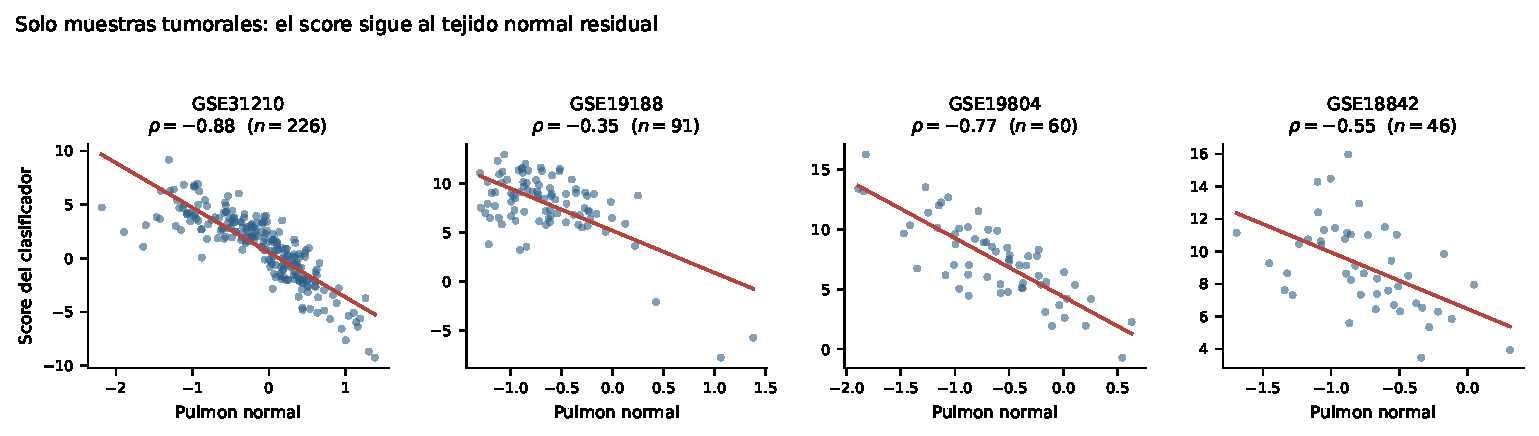
\includegraphics[width=\textwidth]{figuras_auditoria/fig_composicion_tumores.pdf}
\caption[Composición tisular dentro de los tumores]{Relación entre el
\emph{score} del clasificador y el contenido estimado de pulmón normal,
restringida a muestras tumorales. La pendiente negativa persiste al eliminar los
controles sanos, lo que indica que parte de la señal procede de tejido normal
residual y no de biología tumoral.}
\label{fig:composicion}
\end{figure}

\subsection{Validez de la consistencia de signo como medida de reproducibilidad}
\label{sec:falacia}

El análisis original cuantificaba la estabilidad de cada gen sumando el signo de
su coeficiente a lo largo de los \emph{folds} LODO, y presentaba valores como
$11/11$ como evidencia de robustez. Esta métrica presenta un problema
estructural: cada \emph{fold} entrena con todas las cohortes menos una, de modo
que dos \emph{folds} cualesquiera comparten la mayor parte de sus muestras de
entrenamiento. En la configuración analizada, la fracción compartida entre pares
de \emph{folds} oscila entre el 62,5\,\% y el 98,5\,\%, con una mediana del
97,6\,\%. No se trata de réplicas independientes, sino del mismo modelo ajustado
varias veces sobre datos casi idénticos.

Se midió el acuerdo direccional de dos formas sobre los mismos genes y las
mismas ocho cohortes: entre \emph{folds} LODO y entre modelos ajustados de forma
independiente en cada cohorte. Los resultados iniciales estaban confundidos por
el tamaño de muestra, dado que los modelos por cohorte disponen de entre 10 y
246 muestras frente a las 416--652 de los \emph{folds}, y con penalización $L_1$
un menor tamaño produce menos genes seleccionados. Se añadió por ello un control
que compara parejas de modelos con entrenamientos de magnitud comparable,
variando únicamente el solapamiento entre ellos.

\begin{table}[htbp]
\centering
\caption[Consistencia de signo: folds solapados frente a cohortes disjuntas]{
Acuerdo direccional de los coeficientes LASSO medido de dos formas sobre los
mismos genes y las mismas ocho cohortes. La ultima fila es el control que
descarta el tamano de muestra como explicacion: compara parejas de modelos con
entrenamientos de magnitud comparable, y unicamente cambia si comparten muestras.}
\label{tab:falacia}
\small
\begin{tabular}{lcc}
\toprule
& \emph{Folds} LODO & Cohortes \\
& (solapados) & (disjuntas) \\
\midrule
Muestras de entrenamiento compartidas & $\sim$98\,\% & 0\,\% \\
Genes seleccionados alguna vez & 724 & 309 \\
Genes seleccionados en las 8 & 10 & 0 \\
Genes con acuerdo de signo perfecto & \textbf{10} & \textbf{0} \\
\midrule
\emph{Control}: concordancia entre parejas & \textbf{100,0\,\%} & \textbf{74,0\,\%} \\
\bottomrule
\end{tabular}
\end{table}


La hipótesis se confirmó, y el control descarta la explicación alternativa. Las
28 parejas de \emph{folds} LODO presentan una concordancia de signo del
\conclodo\,\% --- perfecta, en todos los pares sin excepción ---, mientras que
parejas de mitades disjuntas de tamaño comparable ($n\approx328$ cada una)
concuerdan al \concdisjunta\,\%. La caída de \caidaconc{} puntos es atribuible al solapamiento y
no a la esparsidad del modelo. Una métrica que no puede tomar valores bajos no
aporta información: la consistencia de signo entre \emph{folds} LODO mide la
reproducibilidad del procedimiento de ajuste, no la del fenómeno biológico.

\begin{figure}[htbp]
\centering
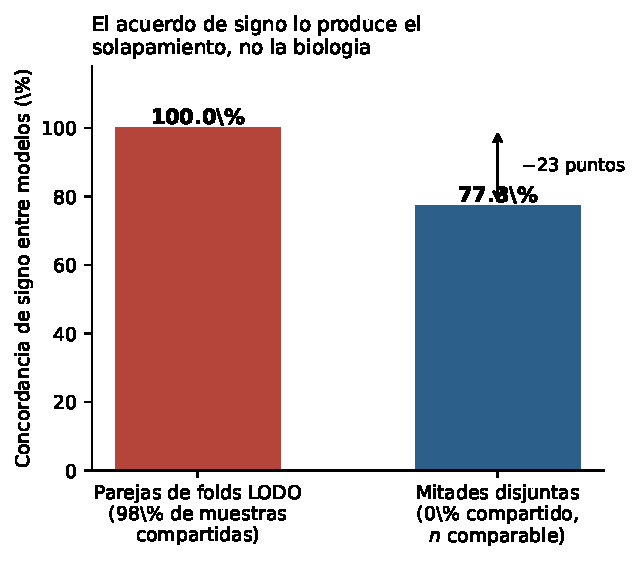
\includegraphics[width=0.58\textwidth]{figuras_auditoria/fig_concordancia_folds.pdf}
\caption[Concordancia de signo y solapamiento]{Concordancia direccional entre
parejas de modelos con entrenamientos de tamaño comparable. La única variable
que cambia entre ambas columnas es la fracción de muestras compartidas.}
\label{fig:falacia}
\end{figure}

La consecuencia sobre la firma previa es directa. De los siete genes destacados
por esta métrica --- SLC6A4, S100A10, KANK3, SH3GL3, HIST1H2BM, ZNF702P y
TOX3 ---, \textbf{ninguno} mantiene coeficiente no nulo y signo constante al
ajustar modelos independientes en las ocho cohortes disjuntas. HIST1H2BM
ilustra el caso con claridad: alcanza un acuerdo de $8/8$ entre \emph{folds}
solapados y no resulta seleccionado en ninguna cohorte individual.

\subsection{Control positivo: clasificación de subtipo histológico}
\label{sec:subtipo}

Los resultados anteriores plantean una pregunta necesaria: si el marco
metodológico no detecta señal reproducible en la tarea tumor frente a sano,
¿está midiendo mal, o simplemente no hay señal que medir? Para distinguir ambas
posibilidades se aplicó el mismo pipeline a una tarea con respuesta conocida y
consecuencia terapéutica real: la distinción entre adenocarcinoma y carcinoma
escamoso, que condiciona la elección de tratamiento --- pemetrexed y
bevacizumab están contraindicados en histología escamosa.

Se emplearon las tres cohortes con histología anotada y ambas clases presentes
(GSE30219, GSE50081 y GSE19188), todas en plataforma GPL570, con 388 muestras y
22\,880 genes comunes. La armonización de códigos requirió atención explícita:
la abreviatura \texttt{SCC} designa carcinoma escamoso en GSE19188 y carcinoma
microcítico en GSE30219, entidades clínicamente opuestas.

\begin{table}[htbp]
\centering
\caption[Control positivo: subtipo histologico]{Validacion LODO de la tarea
adenocarcinoma frente a escamoso sobre las tres cohortes con histologia anotada
y ambas clases presentes (todas en plataforma GPL570).}
\label{tab:subtipo}
\small
\begin{tabular}{lrcrrrr}
\toprule
Cohorte test & $n$ & ADC/Esc. & \emph{Baseline} & Bal.\ acc. & AUC & Ganancia \\
\midrule
GSE30219 & 146 & 85/61 & 0,582 & 0,967 & 0,993 & $+$0,390 \\
GSE50081 & 170 & 127/43 & 0,747 & 0,887 & 0,909 & $+$0,165 \\
GSE19188 & 72 & 45/27 & 0,625 & 0,967 & 0,998 & $+$0,333 \\
\midrule
\multicolumn{4}{l}{\emph{Media}} &
\textbf{0,940} &
\textbf{0,967} &
$+$0,296 \\
\bottomrule
\end{tabular}
\end{table}


El rendimiento es sustancialmente superior al de la tarea tumor frente a sano:
\emph{balanced accuracy} media de \balaccsub{} y AUC media de \aucsub{}, con una ganancia
media de $+$\gananciasub{} sobre el azar informado. Se derivó además una firma de \ngenesfirma{}
genes con $|d|>0{,}8$ y signo concordante en las tres cohortes calculadas de
forma independiente.

La validación más relevante de este resultado no es su magnitud, sino su
contenido. La firma recupera los doce marcadores empleados en inmunohistoquímica
diagnóstica en la práctica clínica, todos en la dirección correcta: siete de
siete para histología escamosa (KRT5, KRT6A, TP63, DSG3, SOX2, PKP1, KRT14) y
cinco de cinco para adenocarcinoma (NAPSA, NKX2-1, SFTPB, SLC34A2, MUC1). Los
primeros puestos del \emph{ranking} --- DSG3, KRT5, CALML3, KRT6B, PKP1, DSC3,
TP63 --- corresponden a desmosomas, queratinas y el programa transcripcional de
TP63, es decir, a linaje celular escamoso y no a composición del tejido.

Este resultado establece que el marco metodológico es capaz de recuperar
biología reproducible cuando existe. Conviene delimitar su alcance: la
distinción entre adenocarcinoma y escamoso está bien caracterizada en la
literatura transcriptómica y su recuperación no constituye un hallazgo nuevo. Su
valor aquí es el de un control positivo, y fue además el análisis que permitió
detectar el desalineamiento descrito en la sección~\ref{sec:auditoria}.

\subsubsection{Límites del clasificador ante histologías no observadas}
\label{sec:dificiles}

El resultado anterior se obtuvo excluyendo \nambiguas{} muestras --- el \pctexcluidas\,\% de los
tumores disponibles --- correspondientes a histologías que no son adenocarcinoma
ni escamoso: neuroendocrino de célula grande, basaloide, carcinoide,
microcítico, célula grande y adenoescamoso. Se excluyeron, por tanto,
precisamente los casos que en la práctica clínica resultan ambiguos. Someter el
modelo a esas muestras es necesario para no sobreestimar su aplicabilidad.

No existe etiqueta correcta que predecir en ellas, de modo que lo evaluado es la
calibración: un modelo prudente debería asignarles probabilidades intermedias.
La métrica fijada de antemano fue el porcentaje de muestras con $P>0{,}9$ o
$P<0{,}1$, y la hipótesis registrada, que superaría el 50\,\%.

\begin{table}[htbp]
\centering
\caption[Histologias excluidas del clasificador de subtipo]{Comportamiento del
clasificador de subtipo ante las histologias que no vio en el entrenamiento
(grupos con $n\geq3$). \emph{Alta conf.} recoge el porcentaje de muestras con
$P>0{,}9$ o $P<0{,}1$, es decir, asignadas con confianza a una categoria a la
que no pertenecen.}
\label{tab:dificiles}
\small
\begin{tabular}{llrrrr}
\toprule
Histologia & Cohorte & $n$ & $P$(esc.) mediana & Alta conf. & A escamoso \\
\midrule
neuroendocrino celula grande & GSE30219 & 56 & 0,161 & 32,1\,\% & 8,9\,\% \\
basaloide & GSE30219 & 39 & 0,927 & 59,0\,\% & 89,7\,\% \\
carcinoide & GSE30219 & 24 & 0,173 & 8,3\,\% & 4,2\,\% \\
microcitico (small cell) & GSE30219 & 21 & 0,272 & 9,5\,\% & 4,8\,\% \\
celula grande & GSE19188 & 19 & 0,409 & 10,5\,\% & 31,6\,\% \\
celula grande & GSE50081 & 7 & 0,236 & 28,6\,\% & 42,9\,\% \\
otro & GSE30219 & 4 & 0,392 & 50,0\,\% & 50,0\,\% \\
celula grande & GSE30219 & 3 & 0,106 & 33,3\,\% & 0,0\,\% \\
\bottomrule
\end{tabular}
\end{table}


\textbf{La hipótesis no se confirmó.} Solo el \pctconfambiguas\,\% de las muestras ambiguas
recibe una asignación de alta confianza, frente al \pctconfvistas\,\% de las muestras que
sí pertenecen a alguna de las dos clases. El modelo es, por tanto, más prudente
ante lo que no ha visto de lo que se había previsto.

El valor agregado oculta, sin embargo, dos comportamientos opuestos que la
figura~\ref{fig:dificiles} separa. El carcinoma basaloide recibe una mediana de
$P(\text{escamoso})=0{,}937$ y se asigna a escamoso en el 89,7\,\% de los casos;
esto no constituye necesariamente un error, dado que varias clasificaciones lo
consideran una variante de carcinoma escamoso, de modo que el modelo puede estar
recuperando la biología correcta. En cambio, de los \nneuro{} tumores neuroendocrinos
(neuroendocrino de célula grande, microcítico y carcinoide), el \pctneuroadc\,\% se asigna
a adenocarcinoma. Este sí es un fallo con consecuencia clínica directa: el
carcinoma microcítico recibe un tratamiento completamente distinto al del cáncer
de pulmón no microcítico, y el modelo lo etiqueta como adenocarcinoma sin
señalar incertidumbre.

\begin{figure}[htbp]
\centering
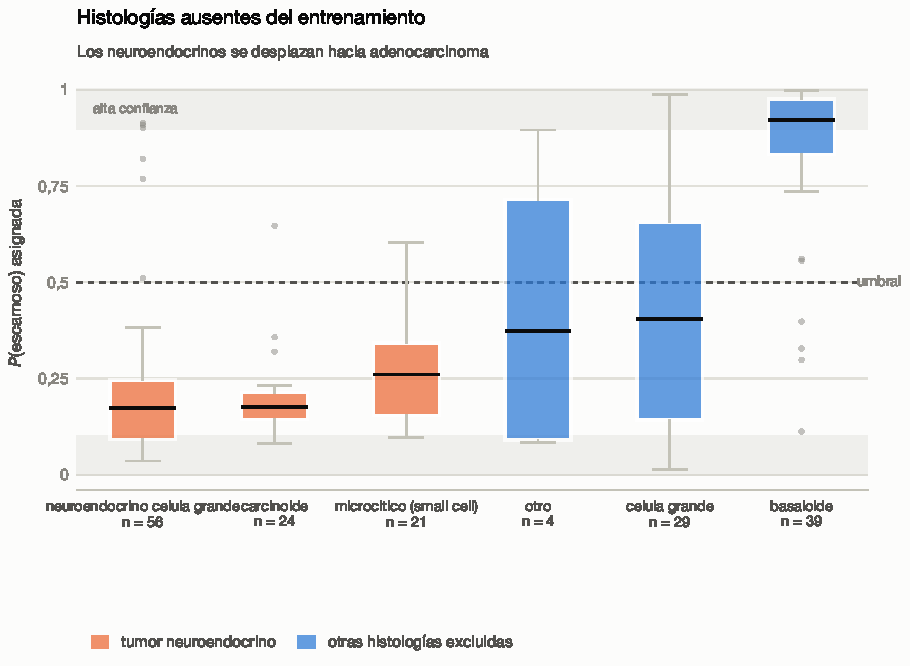
\includegraphics[width=0.95\textwidth]{figuras_auditoria/fig_histologias_excluidas.pdf}
\caption[Histologías excluidas del entrenamiento]{Distribución de la
probabilidad asignada a las histologías ausentes del entrenamiento. En rojo, los
tumores neuroendocrinos, desplazados hacia adenocarcinoma. Las bandas grises
delimitan las regiones de alta confianza.}
\label{fig:dificiles}
\end{figure}

El AUC de \aucsub{} de la sección~\ref{sec:subtipo} es válido únicamente sobre
tumores previamente confirmados como adenocarcinoma o escamoso. El modelo no
puede emplearse como primer filtro sobre un caso sin diagnosticar.

\subsection{Síntesis de resultados}
\label{sec:sintesis}

Los cinco análisis permiten establecer lo siguiente:

\begin{enumerate}
\item Los datos presentan cuatro modos de fallo silencioso y cuantificables:
      tres cohortes declaradas nunca procesadas, \ndesalineadas{} muestras con etiqueta
      cruzada, \sinclasificar{} muestras (\pctsinclasificar\,\%) perdidas en la curación automatizada y
      \nmonoclase{} cohortes de una sola clase empleadas como conjunto de test. Ninguno
      generó un error en tiempo de ejecución.
\item En la tarea tumor frente a sano, la \emph{balanced accuracy} media sobre
      cohortes evaluables es de \balacc{}, con \nosuperan{} de \nev{} por debajo de su propio
      \emph{baseline}.
\item La firma transfiere su capacidad de ordenación entre cohortes (AUC medio
      \aucmedia{}) pero no su umbral de decisión (especificidad media \especmedia{}), un
      problema de calibración inducido por el desbalance del entrenamiento.
\item La composición tisular explica una parte sustancial de la señal
      ($\rho=-\rhotumoresabs$ entre tumores) sin agotarla, y coexiste con un eje de
      proliferación no previsto.
\item La consistencia de signo entre \emph{folds} LODO no mide reproducibilidad
      biológica: alcanza el \conclodo\,\% frente al \concdisjunta\,\% de modelos disjuntos
      comparables, y ninguno de los siete genes destacados por esa métrica
      replica de forma independiente.
\item El marco metodológico sí recupera biología reproducible cuando existe
      (subtipo histológico, AUC \aucsub{}, con los doce marcadores de
      inmunohistoquímica recuperados), con la limitación de no reconocer las
      histologías ausentes del entrenamiento.
\end{enumerate}


\clearpage
% =====================================================================
% CAPITULO 6 - DISCUSION
% Sustituye al capitulo 6 de la version anterior de la memoria.
% =====================================================================

\section{Discusión}
\label{cap:discusion}

\subsection{Reorientación del objeto de estudio}
\label{sec:disc-reorientacion}

El planteamiento inicial de este trabajo perseguía identificar biomarcadores
transcriptómicos universales de cáncer de pulmón mediante la integración de
múltiples cohortes públicas. Los resultados del capítulo anterior no sostienen
ese objetivo, y conviene ser explícito sobre por qué.

La firma derivada del contraste entre tejido tumoral y tejido sano adyacente
reúne tres características que impiden interpretarla como un conjunto de
biomarcadores: su señal procede en parte sustancial de la composición del tejido
más que de biología tumoral específica (sección~\ref{sec:composicion}); su
estabilidad aparente era un artefacto del diseño de validación
(sección~\ref{sec:falacia}); y la tarea que resuelve no constituye un problema
clínico, dado que la distinción entre tumor y parénquima normal la resuelve el
examen histopatológico convencional con fiabilidad superior, coste
incomparablemente menor y sobre la misma muestra ya disponible.

Esto no invalida el framework desarrollado. Lo que invalida es la lectura que se
había hecho de sus resultados. El pipeline descarga, normaliza, curó
metadatos mediante modelos de lenguaje, ejecuta análisis diferencial, entrena
modelos y valida de forma externa; todos esos componentes funcionan, y el
control positivo de la sección~\ref{sec:subtipo} demuestra que recuperan biología
reproducible cuando está presente. La contribución defendible de este trabajo no
es, por tanto, una firma molecular, sino la caracterización sistemática de los
modos en que estos pipelines fallan sin avisar, y un conjunto de controles
concretos para detectarlos.

\subsection{Los cuatro modos de fallo silencioso}
\label{sec:disc-fallos}

Los problemas documentados en la sección~\ref{sec:auditoria} comparten un rasgo
que los hace especialmente peligrosos: ninguno interrumpe la ejecución. El
pipeline termina, escribe sus ficheros y produce tablas de aspecto correcto.

\paragraph{El desalineamiento como fallo indistinguible.} El caso de GSE30219 es
instructivo porque su efecto imita exactamente el de una hipótesis nula
verdadera. Un AUC de 0,56 sobre una cohorte de 146 tumores es perfectamente
compatible con la conclusión «esta señal no generaliza a esta cohorte», y ese es
el tipo de resultado que un trabajo honesto acepta y reporta. Solo la
comparación con marcadores de referencia externos --- la observación de que KRT5
mostraba una diferencia de $+0{,}90$ en esta cohorte frente a $+5{,}32$ y
$+5{,}66$ en las otras dos --- reveló que la señal estaba presente pero
desacoplada de las etiquetas. La lección metodológica es que la validación
frente a conocimiento biológico previo no es un adorno interpretativo, sino un
control de integridad de los datos.

Resulta pertinente señalar que el análisis original no se vio afectado por este
error, y la razón es instructiva: GSE30219 contiene una sola clase, de modo que
intercambiar etiquetas idénticas entre sí no altera nada. El fallo permaneció
latente y solo se manifestó al plantear una pregunta que utilizara la
información clínica. Un pipeline puede arrastrar errores de este tipo durante
todo su ciclo de vida sin que se manifiesten, hasta que alguien formula la
pregunta adecuada.

\paragraph{La curación automatizada como fuente de sesgo de selección.} El
empleo de modelos de lenguaje para homogeneizar metadatos clínicos heterogéneos
es una de las aportaciones metodológicamente más interesantes del framework, y
su comportamiento bimodal --- éxito prácticamente completo en ocho cohortes,
colapso en dos --- merece una lectura cuidadosa. El problema no es la tasa
global del 82,8\,\%, sino que las pérdidas no son aleatorias: se concentran en
cohortes concretas y, dentro de ellas, afectan a la práctica totalidad de las
muestras. GSE40791 pasó de 194 muestras a 12, y las 12 supervivientes presentan
una composición de clases (10 controles y 2 tumores) que no representa al
estudio original. El resultado es un sesgo de selección introducido por una capa
de procesamiento automático, no declarado como tal en ningún punto del
pipeline. La recomendación que se deriva es que cualquier etapa de curación
automatizada debe reportar su tasa de éxito por cohorte como parte de los
resultados, y que las cohortes con tasas bajas deben excluirse explícitamente en
lugar de participar con su fracción superviviente.

\paragraph{Cohortes de una sola clase.} Que GSE30219 y GSE50081 no contengan
controles no es un defecto de esas cohortes: son estudios de supervivencia,
diseñados para correlacionar expresión con evolución clínica, y su composición es
la correcta para su propósito. El error consiste en emplearlas como conjunto de
test de un clasificador binario. Este fallo es además el más fácil de detectar
automáticamente --- basta comprobar el número de clases presentes antes de
evaluar --- y el más fácil de pasar por alto cuando la métrica reportada es
únicamente la \emph{accuracy}, porque produce precisamente los valores más altos
de la tabla.

\subsection{Discriminación y decisión como propiedades independientes}
\label{sec:disc-calibracion}

El hallazgo de la sección~\ref{sec:calibracion} no estaba previsto y es, a
nuestro juicio, el resultado de mayor utilidad práctica del trabajo. La
coexistencia de un AUC medio de 0,925 con una \emph{balanced accuracy} media de
0,773, y su expresión extrema en GSE40791 (\emph{accuracy} 0,167 con AUC 1,000),
descompone lo que habitualmente se trata como un único atributo --- «el modelo
generaliza» o «no generaliza» --- en dos propiedades que transfieren de forma
independiente entre cohortes.

La capacidad de ordenación transfiere bien: la firma sitúa consistentemente las
muestras tumorales por encima de los controles en cohortes que nunca ha visto. El
umbral de decisión no transfiere: el punto de corte aprendido sobre una
distribución de clases determinada (938 tumores frente a 219 controles) deja de
ser adecuado cuando la cohorte de destino presenta otra composición. La
sensibilidad media de 0,983 frente a una especificidad media de 0,563 describe un
modelo que ha aprendido, razonablemente dada su dieta de entrenamiento, que
predecir «tumor» casi siempre acierta.

Esta lectura reinterpreta un patrón que el análisis original registraba sin
explicar. Los casos de \emph{accuracy} próxima a 0,5 acompañada de AUC próximo a
1,0 se habían atribuido a la dificultad intrínseca del problema, al tamaño
muestral reducido o a particularidades técnicas de los estudios. No era ninguna
de esas cosas: era un problema de calibración, y los problemas de calibración
son corregibles. La vía inmediata es la ponderación de clases en el
entrenamiento; la más robusta, reportar métricas independientes del umbral (AUC,
precisión media) junto con métricas de decisión, y ajustar el punto de corte
sobre la cohorte de destino cuando el escenario de aplicación lo permita.

\subsection{Qué mide la firma: composición, proliferación y biología}
\label{sec:disc-composicion}

La hipótesis de que la firma tumor frente a sano capturase esencialmente
composición tisular no se confirmó al umbral fijado de antemano
($|\rho|>0{,}7$; obtenido $\rho=-0{,}637$). Mantener ese criterio obliga a una
conclusión más matizada, y probablemente más correcta, que la hipótesis de
partida.

La composición tisular explica una fracción sustancial de la señal. La evidencia
es convergente: la correlación entre el \emph{score} del clasificador y el
contenido de pulmón normal persiste al restringir el análisis a muestras
tumorales, alcanzando $\rho=-0{,}870$ ($p=7\times10^{-71}$) en la cohorte con
mayor número de tumores evaluables; y cinco de los cincuenta genes principales de
la firma son marcadores canónicos de epitelio alveolar y estroma pulmonar normal,
con $\log$FC en torno a $-4$. Interpretados como biomarcadores tumorales, genes
como AGER, CLDN18 o SFTPC informan principalmente de cuánto parénquima sano
conserva la muestra.

Pero no la agotan. El segundo eje detectado --- correlación positiva con
proliferación, entre $+0{,}267$ y $+0{,}719$ --- indica que el clasificador
integra al menos dos fenómenos distintos, y el segundo sí es biología tumoral en
sentido estricto. La descripción más ajustada de lo que mide la firma es
«pérdida de arquitectura alvéolo-capilar normal más ganancia de actividad
proliferativa», una combinación real, reproducible y de escaso valor
discriminativo por ser común a la práctica totalidad de los tumores sólidos.

Debe señalarse una limitación de este análisis: solo cuatro cohortes reunían
tumores suficientes ($n\geq8$) para el contraste restringido, y los estimadores
presentan heterogeneidad notable entre ellas ($\rho$ de $-0{,}343$ a
$-0{,}870$). Un abordaje más riguroso emplearía métodos de deconvolución celular
para estimar la proporción de cada tipo celular, en lugar de un panel de
marcadores promediado.

\subsection{Implicaciones sobre el diseño de la validación externa}
\label{sec:disc-lodo}

La estrategia LODO es metodológicamente superior a la validación cruzada
convencional dentro de un mismo estudio, y su adopción sigue siendo escasa en la
literatura de biomarcadores transcriptómicos. Este trabajo no cuestiona esa
elección, sino dos usos concretos que se hicieron de ella.

El primero es de terminología con consecuencias conceptuales: LODO no corrige el
efecto lote, lo \emph{mide}. Presentarla como mecanismo de superación del
\emph{batch effect} confunde la naturaleza del procedimiento. En el pipeline
analizado no existe corrección de lote alguna --- solo normalización por
cuantiles dentro de cada estudio y estandarización por estudio ---, y la
degradación de rendimiento entre cohortes que LODO revela \emph{es} la magnitud
del problema, no su solución.

El segundo es el uso de los \emph{folds} LODO como réplicas para medir
estabilidad. La demostración de la sección~\ref{sec:falacia} es cuantitativa y,
en nuestra opinión, generalizable más allá de este trabajo: cuando el número de
cohortes es moderado, los conjuntos de entrenamiento de los distintos
\emph{folds} comparten una mediana del 97,6\,\% de sus muestras, y la
concordancia direccional resultante es del 100,0\,\% en la totalidad de los
pares. Una métrica cuyo valor está determinado por el diseño no puede aportar
evidencia sobre el fenómeno estudiado. El control con mitades disjuntas de
tamaño comparable (73,98\,\%) delimita cuánto de ese 100\,\% procede del
solapamiento.

La consecuencia sobre los siete genes previamente destacados es contundente:
ninguno replica al ajustar modelos independientes. Esto no significa que carezcan
de interés biológico --- SLC6A4 y KANK3 son marcadores endoteliales pulmonares
bien caracterizados, coherentes con la interpretación composicional de la
sección anterior ---, sino que la evidencia aportada para priorizarlos no era
evidencia. La alternativa empleada en la sección~\ref{sec:subtipo}, exigir
concordancia de tamaño de efecto en cohortes ajustadas por separado, es más
exigente y produjo una firma que recupera marcadores de uso clínico establecido.

\subsection{Alcance y limitaciones del control positivo}
\label{sec:disc-subtipo}

La clasificación de subtipo histológico cumple su función como control positivo:
demuestra que el marco metodológico detecta biología reproducible cuando existe,
con AUC medio de 0,967 y recuperación completa de los doce marcadores de
inmunohistoquímica diagnóstica. Conviene, no obstante, precisar tres límites.

Primero, la distinción entre adenocarcinoma y carcinoma escamoso está
extensamente caracterizada en transcriptómica y su recuperación no constituye una
aportación original. Su valor es de verificación, no de descubrimiento.

Segundo, el resultado se obtuvo excluyendo el 31,3\,\% de los tumores
disponibles, precisamente los de histología ambigua. El análisis de la
sección~\ref{sec:dificiles} muestra que el modelo es más prudente ante esas
muestras de lo previsto (29,9\,\% de asignaciones de alta confianza frente al
62,6\,\% en muestras de clase conocida; la hipótesis registrada no se confirmó),
pero también que el 93\,\% de los 101 tumores neuroendocrinos se etiqueta como
adenocarcinoma. Dado que el carcinoma microcítico requiere un abordaje
terapéutico completamente distinto, esta es una limitación con consecuencia
clínica y no meramente estadística.

Tercero, las tres cohortes comparten plataforma (GPL570), de modo que el
resultado no informa sobre transferencia entre tecnologías de medición. Las tres
cohortes de RNA-seq que habrían permitido evaluarlo son precisamente las que el
pipeline no llegó a procesar.

\subsection{Recomendaciones metodológicas}
\label{sec:disc-recomendaciones}

De los resultados obtenidos se derivan seis controles concretos, aplicables a
cualquier pipeline de descubrimiento de biomarcadores sobre repositorios
públicos:

\begin{enumerate}
\item \textbf{Alinear muestras y metadatos por identificador explícito}, nunca
      por posición, y verificar la correspondencia como paso previo a cualquier
      análisis. La coincidencia de longitudes no implica coincidencia de orden.
\item \textbf{Validar contra marcadores biológicos conocidos} antes de
      interpretar cualquier resultado. Un panel de referencia de la patología
      estudiada funciona como control de integridad de los datos y detecta
      fallos que ninguna comprobación de formato revela.
\item \textbf{Reportar el \emph{baseline} de clase mayoritaria} junto a toda
      métrica de rendimiento, y excluir explícitamente las cohortes de una sola
      clase de la evaluación, indicándolo en las tablas.
\item \textbf{Separar métricas de discriminación y de decisión.} Informar AUC y
      \emph{balanced accuracy} conjuntamente, con sensibilidad y especificidad
      desglosadas; su divergencia identifica problemas de calibración que la
      \emph{accuracy} agregada oculta.
\item \textbf{Medir la estabilidad sobre particiones disjuntas}, no sobre
      \emph{folds} solapados, y declarar la fracción de muestras compartidas
      cuando se empleen estas últimas.
\item \textbf{Cuantificar y reportar la tasa de éxito de toda etapa de curación
      automatizada} por cohorte, tratando las pérdidas elevadas como criterio de
      exclusión y no como merma silenciosa del tamaño muestral.
\end{enumerate}

\subsection{Líneas futuras}
\label{sec:disc-futuro}

Los datos ya descargados permiten abordar preguntas que este trabajo no ha
explorado y que resultan más informativas que la comparación entre tumor y tejido
sano. GSE30219 y GSE50081 disponen de seguimiento clínico completo (307 y 181
tumores, con 200 y 75 eventos de mortalidad respectivamente), lo que habilita
análisis de supervivencia con validación cruzada entre cohortes. GSE31210
incluye el estado de los principales genes conductores --- 127 tumores con
mutación de EGFR, 20 de KRAS, 11 con fusión de ALK y 68 sin ninguna de las tres
alteraciones ---, lo que permite plantear la predicción de alteración
conductora a partir del perfil de expresión. Ambas son preguntas cuya respuesta
no se conoce de antemano por inspección de la muestra, condición que la tarea
tumor frente a sano no cumplía.

En el plano metodológico, tres extensiones mejorarían el rigor de los análisis
presentados: el empleo de deconvolución celular en lugar de paneles de
marcadores promediados para cuantificar composición tisular; la incorporación de
corrección de lote explícita, con evaluación de su efecto sobre la transferencia
entre cohortes; y la recuperación de las tres cohortes de RNA-seq no procesadas,
que permitirían por primera vez evaluar la generalización entre plataformas de
medición distintas.


\end{document}
